\documentclass[aspectratio=169, 11pt]{beamer}

\usepackage[T1]{fontenc}
\usepackage[utf8]{inputenc}
\usepackage[spanish, es-tabla]{babel}
\usepackage[scaled=0.94]{helvet}
\usepackage{graphicx}
\usepackage{tikz}
\usetikzlibrary{positioning, arrows.meta, fadings, calc}
\usepackage{amsmath}
\usepackage[gen]{eurosym}

\graphicspath{{imagenes/}{../imagenes/}{./}}
% Tema de la presentación. Toma los colores de la propia aplicación, que es
% oscura, para que las capturas no queden como recuadros negros flotando sobre
% blanco y el conjunto se lea como una sola cosa.

\usetheme{default}
\usecolortheme{default}
\setbeamertemplate{navigation symbols}{}

% Paleta copiada de frontend/src/index.css y de la de grupos de App.jsx.
\definecolor{fondo}{HTML}{0B0C0E}
\definecolor{superficie}{HTML}{14171B}
\definecolor{superficiedos}{HTML}{1B1F25}
\definecolor{linea}{HTML}{2A2F36}
\definecolor{texto}{HTML}{E8E9EB}
\definecolor{apagado}{HTML}{8E949D}
\definecolor{tenue}{HTML}{565C64}
\definecolor{acento}{HTML}{4C7DF0}
\definecolor{acentoclaro}{HTML}{6F97F5}
\definecolor{verde}{HTML}{58C4A3}
\definecolor{ambar}{HTML}{E0A458}
\definecolor{rojo}{HTML}{D6685E}
\definecolor{morado}{HTML}{A98BD0}

\setbeamercolor{background canvas}{bg=fondo}
\setbeamercolor{normal text}{fg=texto, bg=fondo}
\setbeamercolor{structure}{fg=acento}
\setbeamercolor{alerted text}{fg=acentoclaro}
\setbeamercolor{frametitle}{fg=texto, bg=fondo}
\setbeamercolor{itemize item}{fg=acento}
\setbeamercolor{enumerate item}{fg=acento}

\setbeamerfont{frametitle}{size=\Large, series=\bfseries}
\setbeamerfont{footline}{size=\tiny}

\setbeamertemplate{frametitle}{%
	\vspace{0.5em}\hspace{0.055\paperwidth}%
	\begin{minipage}{0.89\paperwidth}
		\raggedright\usebeamerfont{frametitle}\color{texto}%
		\insertframetitle\par\vspace{0.22em}%
		{\color{acento}\rule{2.6em}{2.5pt}}
	\end{minipage}\par\vspace{0.25em}}

% El número que se muestra es el de página del PDF, que es el que aparece en el
% visor y el que usa el guion. Así no hay dos numeraciones distintas.
\setbeamertemplate{footline}{%
	\hbox{\begin{beamercolorbox}[wd=\paperwidth, ht=1.9ex, dp=1.2ex,
			leftskip=0.055\paperwidth, rightskip=0.055\paperwidth]{}%
		\usebeamerfont{footline}\color{tenue}%
		\hfill\thepage%
	\end{beamercolorbox}}}

\setbeamertemplate{itemize item}{\color{acento}\raisebox{0.15ex}{\rule{0.42em}{0.42em}}}
\setbeamertemplate{itemize subitem}{\color{tenue}\raisebox{0.18ex}{\rule{0.3em}{0.3em}}}
\setbeamertemplate{enumerate item}{\color{acento}\bfseries\insertenumlabel}
\setlength{\leftmargini}{1.3em}

% ---------------------------------------------------------------------------
% Separador de bloque: el número muy grande, en color, y el nombre debajo.
\AtBeginSection[]{%
	\begin{frame}[plain, noframenumbering]
		\vfill
		\hspace{0.09\paperwidth}%
		\begin{minipage}{0.8\paperwidth}
			{\color{acento}\fontsize{72}{72}\selectfont\bfseries\insertsectionnumber}\\[0.25em]
			{\color{texto}\fontsize{26}{30}\selectfont\bfseries\insertsectionhead}\\[0.7em]
			{\color{acento}\rule{3.5em}{2.5pt}}
		\end{minipage}
		\vfill
	\end{frame}}

% ---------------------------------------------------------------------------
% Diapositiva con una captura ocupando toda la superficie.
\newenvironment{lienzo}[1]{%
	\begingroup
	\usebackgroundtemplate{\includegraphics[width=\paperwidth, height=\paperheight]{#1}}%
	\begin{frame}[plain]}%
	{\end{frame}\endgroup}

% Caja de texto que se superpone a una captura. El fondo semitransparente deja
% ver la escena por detrás sin que el texto pierda contraste.
\newcommand{\sobreimagen}[3][north west]{%
	\begin{tikzpicture}[remember picture, overlay]
		\node[anchor=#1, fill=fondo, fill opacity=0.9, text opacity=1, draw=linea,
		      rounded corners=6pt, inner sep=1.1em, text width=0.4\paperwidth, align=left,
		      font=\color{texto}] at ([shift={(#2)}]current page.#1) {#3};
	\end{tikzpicture}}

% Título grande sobre una captura, sin caja.
\newcommand{\tituloimagen}[2]{%
	\begin{tikzpicture}[remember picture, overlay]
		\node[anchor=west, inner sep=0pt] at ([shift={(0.075\paperwidth,0)}]current page.west) {%
			\begin{minipage}{0.55\paperwidth}
				\color{texto}#1\\[0.5em]{\color{acento}\rule{3em}{2.5pt}}\\[0.6em]
				\color{apagado}#2
			\end{minipage}};
	\end{tikzpicture}}

% Velo oscuro para que el texto se lea sobre la captura.
\newcommand{\velo}[1][0.72]{%
	\begin{tikzpicture}[remember picture, overlay]
		\fill[fondo, opacity=#1] (current page.south west) rectangle (current page.north east);
	\end{tikzpicture}}

% Velo solo en la mitad izquierda, degradado, para la portada.
\newcommand{\veloizq}{%
	\begin{tikzpicture}[remember picture, overlay]
		\fill[fondo] (current page.south west) rectangle
			([xshift=0.44\paperwidth]current page.north west);
		\fill[fondo, path fading=east]
			([xshift=0.44\paperwidth]current page.south west) rectangle
			([xshift=0.78\paperwidth]current page.north west);
	\end{tikzpicture}}

% ---------------------------------------------------------------------------
% Tarjeta: bloque con fondo propio para agrupar una idea.
\newcommand{\tarjeta}[3][acento]{%
	\begin{tikzpicture}
		\node[fill=superficie, draw=linea, rounded corners=5pt, inner sep=0.7em,
		      text width=\dimexpr\linewidth-1.9em, align=left] {%
			{\color{#1}\bfseries\small #2}\\[0.3em]{\color{apagado}\footnotesize #3}};
	\end{tikzpicture}}

% Variante de una sola línea, para cuando hay muchas tarjetas juntas.
\newcommand{\tarjetafina}[3][acento]{%
	\begin{tikzpicture}
		\node[fill=superficie, draw=linea, rounded corners=5pt, inner sep=0.6em,
		      text width=\dimexpr\linewidth-1.7em, align=left] {%
			{\color{#1}\bfseries\small #2}\ {\color{apagado}\footnotesize #3}};
	\end{tikzpicture}}

% Cifra destacada con su etiqueta debajo.
\newcommand{\cifra}[3][acento]{%
	\begin{minipage}[t]{0.3\textwidth}\centering
		{\color{#1}\fontsize{30}{32}\selectfont\bfseries #2}\\[0.3em]
		{\color{apagado}\small #3}
	\end{minipage}}

% Los diagramas de la memoria tienen fondo blanco, así que se colocan sobre una
% tarjeta clara en lugar de dejarlos recortados sobre el fondo oscuro.
\newcommand{\diagrama}[2][0.66\textheight]{%
	\begin{tikzpicture}
		\node[fill=white, rounded corners=6pt, inner sep=0.6em]
			{\includegraphics[height=#1, keepaspectratio]{#2}};
	\end{tikzpicture}}

% Rótulo sobre una captura a sangre. Poco texto y bien grande, que es lo que
% se lee desde el fondo de un aula.
\newcommand{\rotulo}[1]{%
	\begin{tikzpicture}[remember picture, overlay]
		\node[anchor=north west, fill=fondo, fill opacity=0.88, text opacity=1, draw=linea,
		      rounded corners=8pt, inner sep=0.9em, align=left, font=\color{texto}]
			at ([shift={(0.05\paperwidth,-0.08\paperheight)}]current page.north west) {#1};
	\end{tikzpicture}}

\newcommand{\rotuloder}[1]{%
	\begin{tikzpicture}[remember picture, overlay]
		\node[anchor=north east, fill=fondo, fill opacity=0.88, text opacity=1, draw=linea,
		      rounded corners=8pt, inner sep=0.9em, align=left, font=\color{texto}]
			at ([shift={(-0.05\paperwidth,-0.08\paperheight)}]current page.north east) {#1};
	\end{tikzpicture}}

% Frase suelta, grande y centrada: una idea por diapositiva.
\newcommand{\frase}[2][texto]{%
	\vfill
	\begin{center}
		\begin{minipage}{0.8\paperwidth}\centering
			{\color{#1}\fontsize{22}{28}\selectfont\bfseries #2}
		\end{minipage}
	\end{center}
	\vfill}

\newcommand{\clave}[1]{{\color{acentoclaro}\bfseries #1}}
\newcommand{\suave}[1]{{\color{apagado}#1}}


\title{Aplicación web para la visualización 3D de redes cerebrales}
\author{Pablo Moliz Arias}
\date{Septiembre de 2026}

\begin{document}

% =========================================================== 1. PORTADA =====
\begingroup
\usebackgroundtemplate{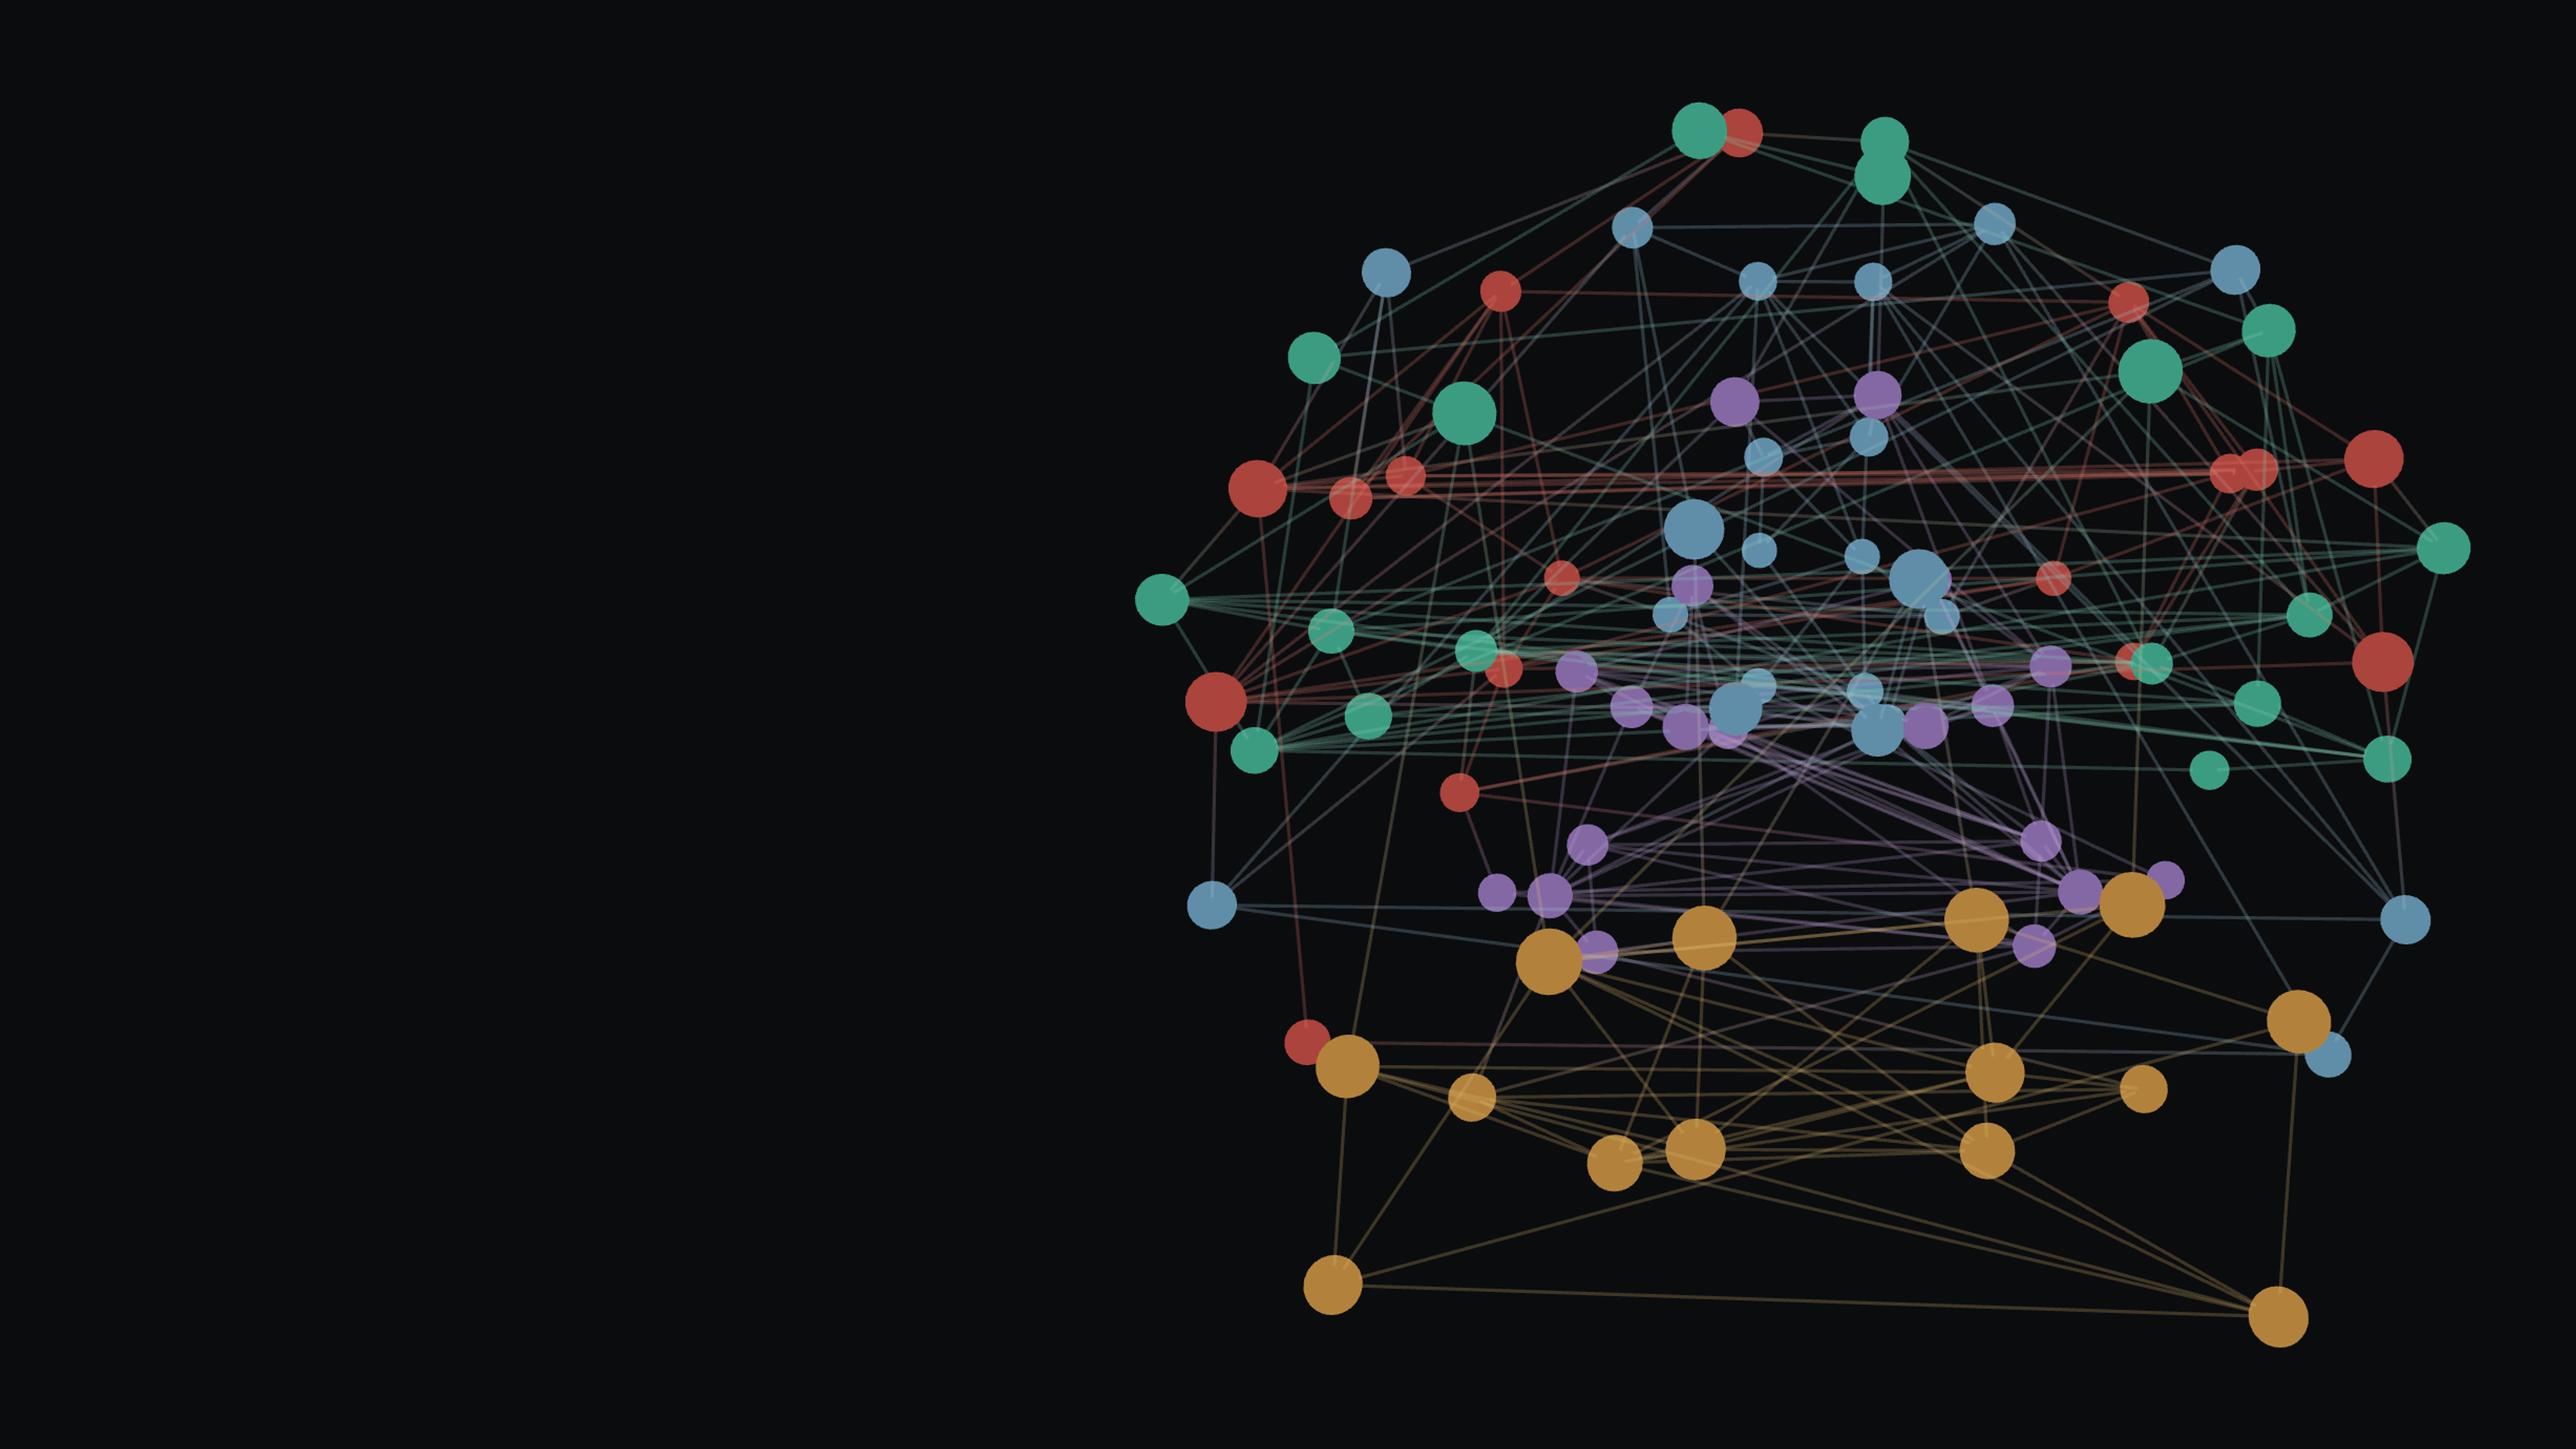
\includegraphics[width=\paperwidth, height=\paperheight]{hero}}
\begin{frame}[plain]
	\veloizq
	\begin{tikzpicture}[remember picture, overlay]
		\node[anchor=west, inner sep=0pt, text width=0.52\paperwidth, align=left]
			at ([shift={(0.075\paperwidth,0.4cm)}]current page.west) {%
			{\color{tenue}\footnotesize TRABAJO FIN DE GRADO}\\[1.0em]
			{\color{texto}\fontsize{25}{30}\selectfont\bfseries Aplicación web para la
			 visualización 3D de redes cerebrales}\\[0.9em]
			{\color{acento}\rule{3.5em}{2.5pt}}\\[0.9em]
			{\color{acentoclaro}\Large\bfseries Brain Viz}\\[1.8em]
			{\color{apagado}\small Pablo Moliz Arias}\\[0.3em]
			{\color{tenue}\small Tutor: Juan Ruiz de Miras}\\[1.2em]
			{\color{tenue}\footnotesize Grado en Ingeniería Informática\\
			 ETSIIT · Universidad de Granada · Septiembre de 2026}};
	\end{tikzpicture}
\end{frame}
\endgroup

% ============================================ 2. EL CEREBRO Y LO QUE HAY =====
\begin{frame}{El cerebro como red, y lo que ya existe}
	\vspace{-0.2em}
	\begin{columns}[c]
		\begin{column}{0.68\textwidth}
			{\footnotesize Cada \clave{región} es un nodo, en sus coordenadas anatómicas. Cada
			\clave{conexión} es una arista con un peso. Sobre esa red hay medidas objetivas: qué
			regiones son puntos de paso, cómo de agrupada está o si se separa en partes.}\\[0.3em]
			{\color{tenue}\scriptsize El atlas AAL90, el ejemplo del trabajo, tiene 90 regiones.}
		\end{column}
		\begin{column}{0.28\textwidth}
			\centering
			\begin{tikzpicture}[scale=0.44,
				nodo/.style={circle, minimum size=5mm, font=\tiny\bfseries, text=fondo, inner sep=0pt}]
				\draw[verde,  line width=1.6pt, opacity=0.75] (0,2.4)--(2.7,3.1);
				\draw[ambar,  line width=1.0pt, opacity=0.75] (2.7,3.1)--(3.3,1.2);
				\draw[rojo,   line width=1.9pt, opacity=0.75] (3.3,1.2)--(1.5,0);
				\draw[morado, line width=0.7pt, opacity=0.75] (1.5,0)--(-0.4,0.9);
				\draw[acento, line width=1.3pt, opacity=0.75] (-0.4,0.9)--(0,2.4);
				\draw[acento, line width=0.9pt, opacity=0.5]  (0,2.4)--(1.5,0);
				\node[nodo, fill=verde]  at (0,2.4)    {R1};
				\node[nodo, fill=ambar]  at (2.7,3.1)  {R2};
				\node[nodo, fill=rojo]   at (3.3,1.2)  {R3};
				\node[nodo, fill=acento] at (1.5,0)    {R4};
				\node[nodo, fill=morado] at (-0.4,0.9) {R5};
			\end{tikzpicture}
		\end{column}
	\end{columns}
	\vspace{0.6em}
	\hspace{0.6em}%
	\begin{minipage}{\textwidth}
		% Rejilla dibujada a mano: las columnas de beamer añaden alto propio y aquí
		% el espacio va justo.
		\begin{tikzpicture}[font=\scriptsize,
			ficha/.style={rounded corners=4pt, draw=linea, fill=superficie, inner sep=0.45em,
			              text width=3.2cm, align=left, minimum height=0.95cm, anchor=north west}]
			\node[text=apagado, anchor=north west] at (0,0.62) {EN EL ESCRITORIO};
			\node[ficha] at (0,0)
				{{\color{ambar}\bfseries BrainNet Viewer}\\ {\color{apagado}depende de MATLAB}};
			\node[ficha] at (3.95,0)
				{{\color{ambar}\bfseries Connectome Workbench}\\ {\color{apagado}formatos propios}};
			\node[ficha] at (7.9,0)
				{{\color{ambar}\bfseries Gephi}\\ {\color{apagado}sin anatomía real}};
			\node[text=apagado, anchor=north west] at (0,-1.35) {YA EN EL NAVEGADOR};
			\node[ficha] at (0,-1.97)
				{{\color{verde}\bfseries Vizaj}\\ {\color{apagado}sin análisis en servidor}};
			\node[ficha] at (3.95,-1.97)
				{{\color{verde}\bfseries BioImage Suite Web}\\ {\color{apagado}un módulo de una suite}};
			\node[ficha] at (7.9,-1.97)
				{{\color{verde}\bfseries Neuroglancer}\\ {\color{apagado}para imagen, no redes}};
		\end{tikzpicture}
	\end{minipage}
\end{frame}

% ============================================ 3. OBJETIVOS Y REQUISITOS =====
\begin{frame}{Objetivos y organización del trabajo}
	\vspace{-0.1em}
	\begin{center}
		\begin{tikzpicture}
			\node[fill=superficie, draw=acento, line width=1pt, rounded corners=6pt,
			      inner sep=0.6em, text width=0.82\paperwidth, align=center] {%
				{\color{apagado}\scriptsize OBJETIVO GENERAL}\ \ {\color{texto}\small Diseñar,
				 desarrollar y desplegar una aplicación web para visualizar y analizar redes
				 cerebrales en 3D.}};
		\end{tikzpicture}
	\end{center}
	\vspace{0.5em}
	\begin{columns}[T]
		\begin{column}{0.56\textwidth}
			{\footnotesize
			\begin{enumerate}
				\setlength{\itemsep}{0.3em}
				\item Cargar y visualizar redes en 3D, en tiempo real.
				\item Analizar la red con métricas de teoría de grafos.
				\item Navegar, filtrar, seleccionar e inspeccionar.
				\item Mantenible, con el procesamiento separado de la vista.
				\item Que se pueda desplegar de manera sencilla.
			\end{enumerate}}
		\end{column}
		\begin{column}{0.4\textwidth}
			\vspace{0.2em}
			\centering
			\cifra{18}{requisitos\\ funcionales}\hfill
			\cifra[verde]{7}{no\\ funcionales}\hfill
			\cifra[ambar]{4}{de\\ información}
		\end{column}
	\end{columns}
	\vspace{0.7em}
	\begin{center}
		\begin{tikzpicture}[font=\scriptsize]
			\foreach \i/\n/\t/\c in {0/1/{ver}/acento, 1/2/{explorar}/verde,
			                         2/3/{analizar}/ambar, 3/4/{usuarios}/morado} {
				\node[fill=superficie, draw=linea, rounded corners=4pt, inner sep=0.45em,
				      minimum width=2.4cm] at (\i*2.9, 0)
					{{\color{\c}\bfseries Sprint \n}\ \ {\color{apagado}\t}};
			}
		\end{tikzpicture}
	\end{center}
\end{frame}

\section{Cómo lo he construido}

% ========================================= 5. ARQUITECTURA Y TECNOLOGÍAS =====
\begin{frame}{Arquitectura y tecnologías}
	\vspace{0.1em}
	\begin{center}
		\begin{tikzpicture}[font=\footnotesize,
			caja/.style={rounded corners=6pt, draw=linea, fill=superficie, inner sep=0.7em,
			             text width=2.9cm, align=center, minimum height=1.5cm},
			flecha/.style={-{Stealth[length=2.5mm]}, acento, line width=1pt}]
			\node[caja] (cli) at (0,0)
				{{\color{acentoclaro}\bfseries Navegador}\\[0.25em]
				 {\color{apagado}\scriptsize React\\ Three.js}};
			\node[caja] (srv) at (5.4,0)
				{{\color{verde}\bfseries Servidor}\\[0.25em]
				 {\color{apagado}\scriptsize Flask\\ NetworkX}};
			\node[caja] (dat) at (10.8,0)
				{{\color{ambar}\bfseries Datos}\\[0.25em]
				 {\color{apagado}\scriptsize Ficheros \texttt{.node} y \texttt{.edge}\\ PostgreSQL}};
			\draw[flecha] (cli) -- node[above, font=\scriptsize, text=apagado] {API REST}
			                       node[below, font=\scriptsize, text=tenue] {JSON} (srv);
			\draw[flecha] (srv) -- node[above, font=\scriptsize, text=apagado] {lee y guarda} (dat);
			
		\end{tikzpicture}
	\end{center}
	\vspace{0.6em}
	\begin{columns}[T]
		\begin{column}{0.31\textwidth}
			\tarjetafina{Flask}{la API es pequeña y de lectura.}\\[0.45em]
			\tarjetafina[verde]{NetworkX}{las métricas del área, contrastadas.}
		\end{column}
		\begin{column}{0.31\textwidth}
			\tarjetafina[acentoclaro]{React}{la interfaz es estado que cambia sin parar.}\\[0.45em]
			\tarjetafina[morado]{react-three-fiber}{la escena 3D se describe como el resto.}
		\end{column}
		\begin{column}{0.31\textwidth}
			\tarjetafina[ambar]{PostgreSQL}{lo subido sobrevive al reinicio.}\\[0.45em]
			\tarjetafina[rojo]{Docker}{la misma imagen en cualquier máquina.}
		\end{column}
	\end{columns}
\end{frame}

% ============================================= 6. SPRINTS 1 Y 2 (UMBRAL) =====
\begingroup
\setbeamertemplate{footline}{}
\begin{frame}[plain]
	\begin{tikzpicture}[remember picture, overlay]
		\begin{scope}
			\clip (current page.north west) rectangle
				([xshift=0.5\paperwidth]current page.south west);
			\node[anchor=north west, inner sep=0pt]
				at ([xshift=-0.25\paperwidth]current page.north west)
				{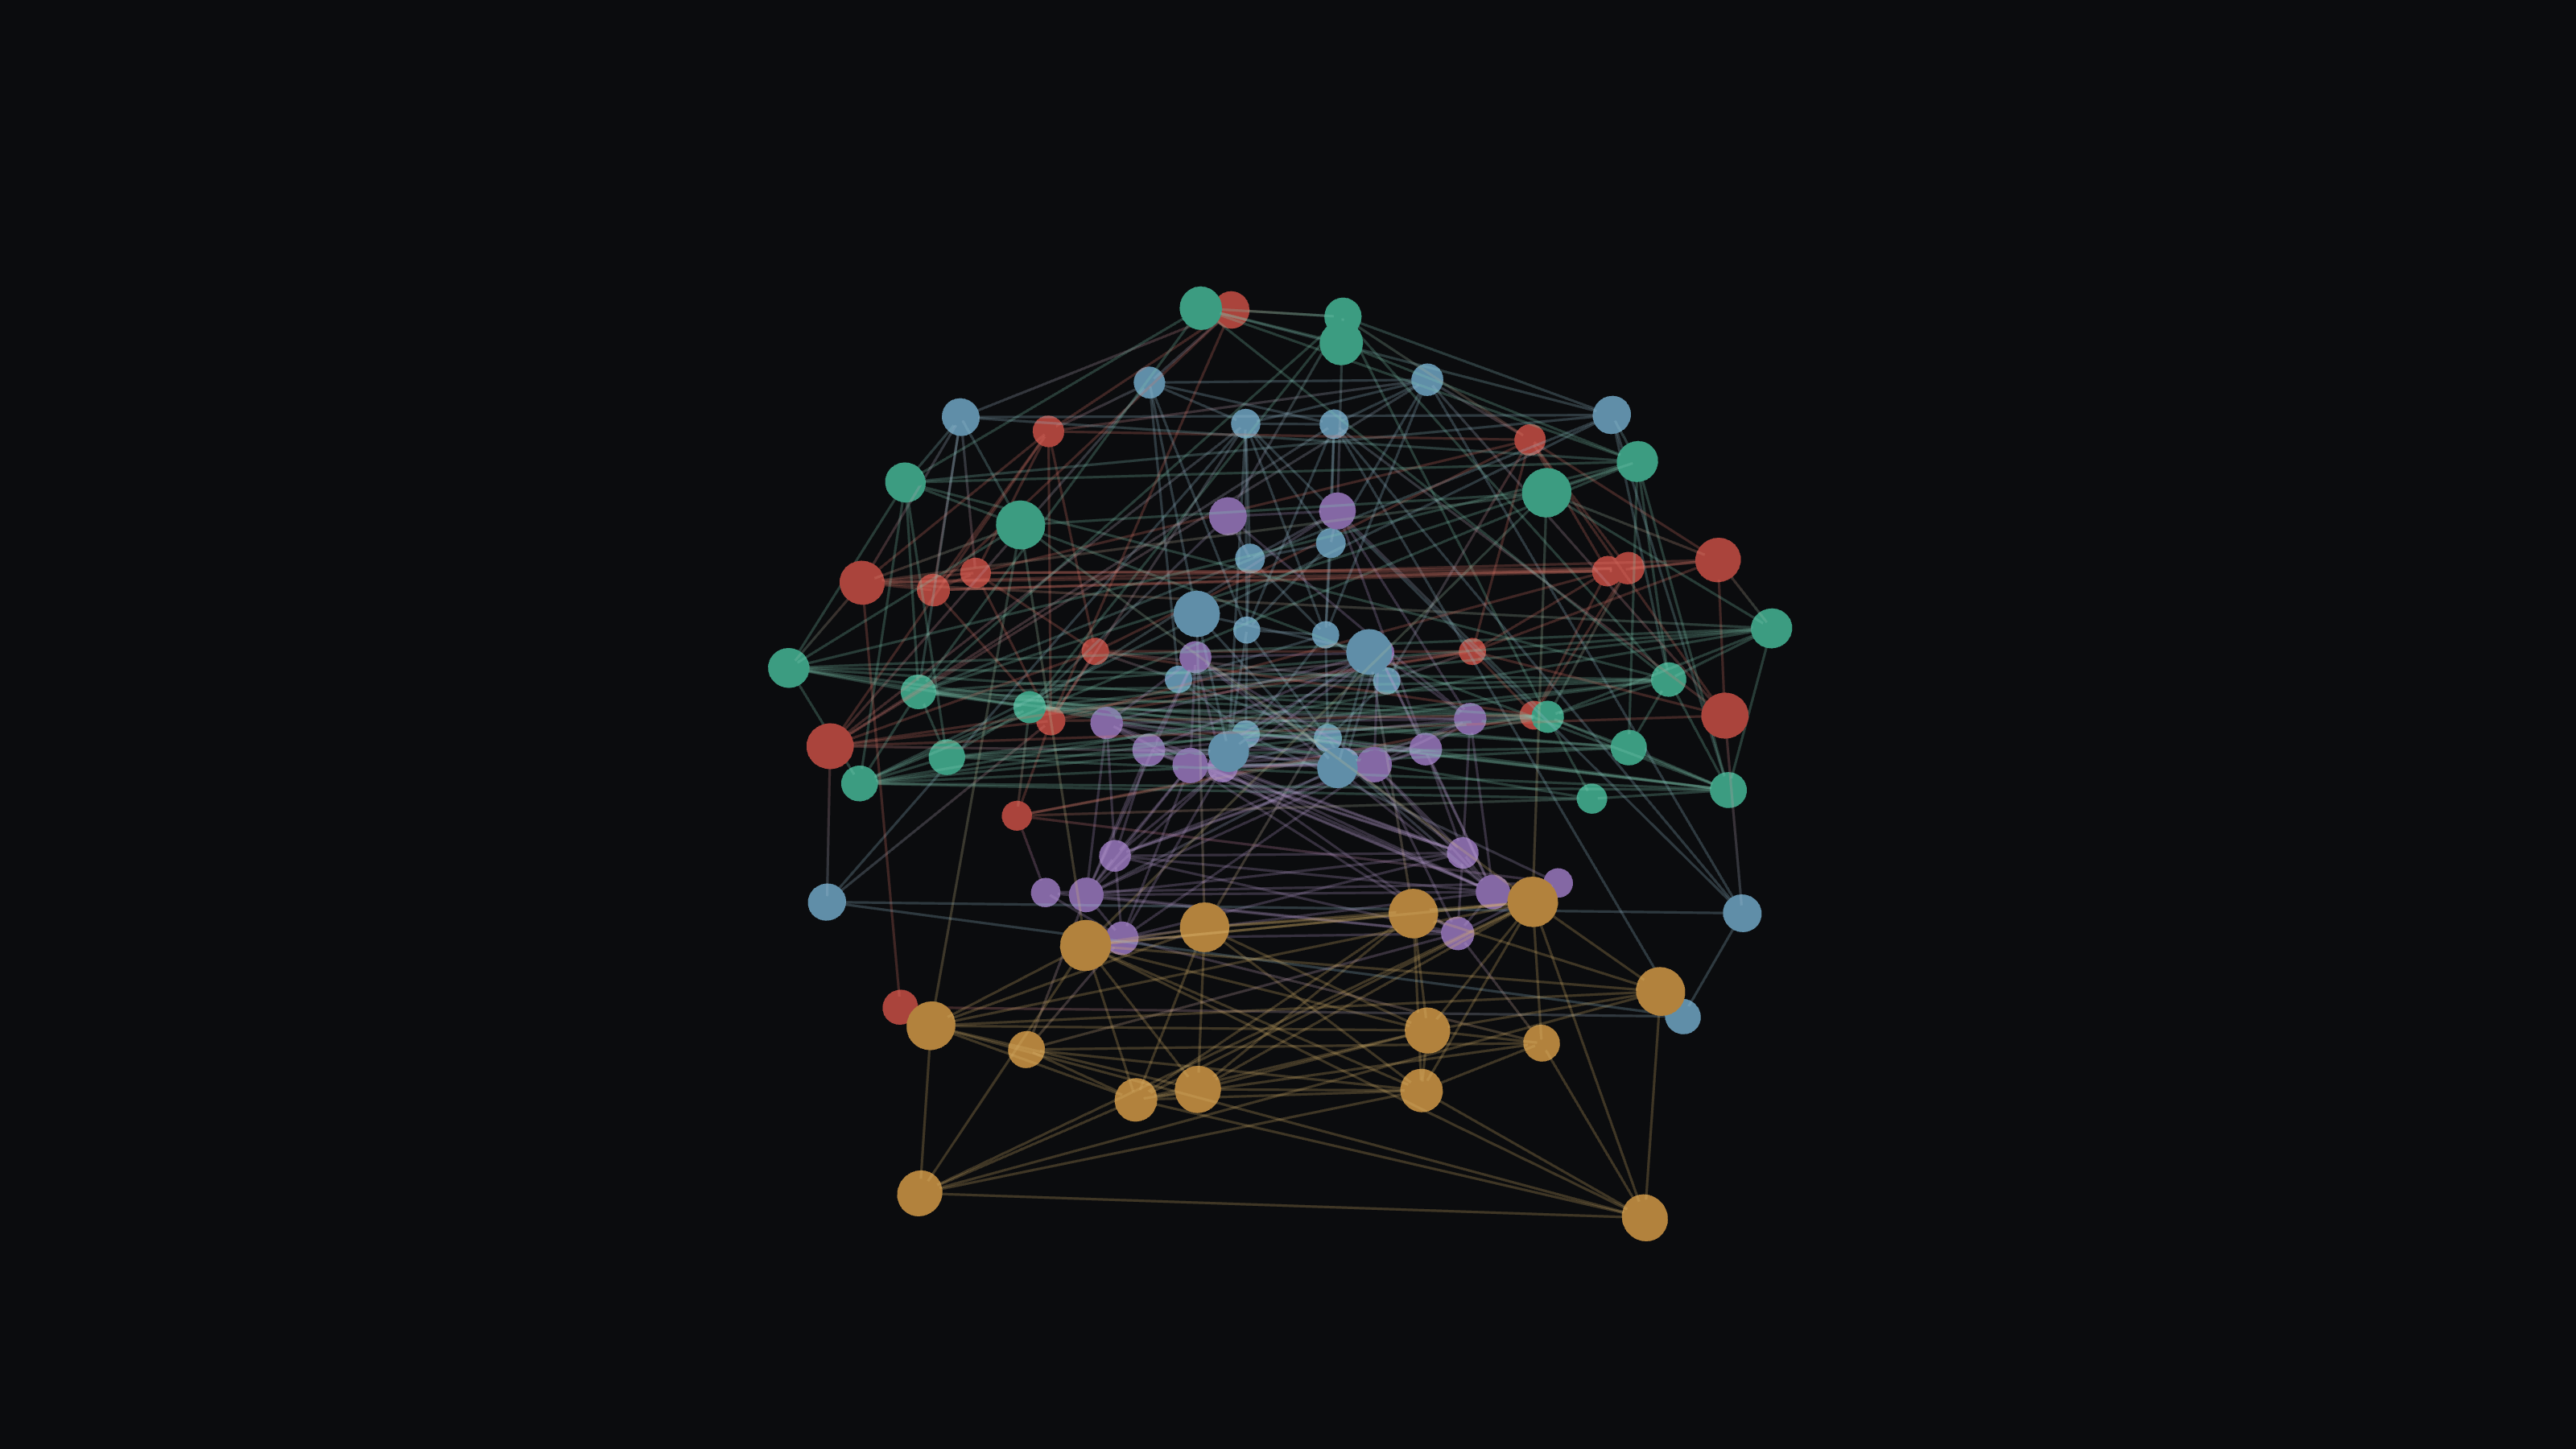
\includegraphics[height=\paperheight]{escena_umbral_0}};
		\end{scope}
		\begin{scope}
			\clip ([xshift=0.5\paperwidth]current page.north west) rectangle
				(current page.south east);
			\node[anchor=north east, inner sep=0pt]
				at ([xshift=0.25\paperwidth]current page.north east)
				{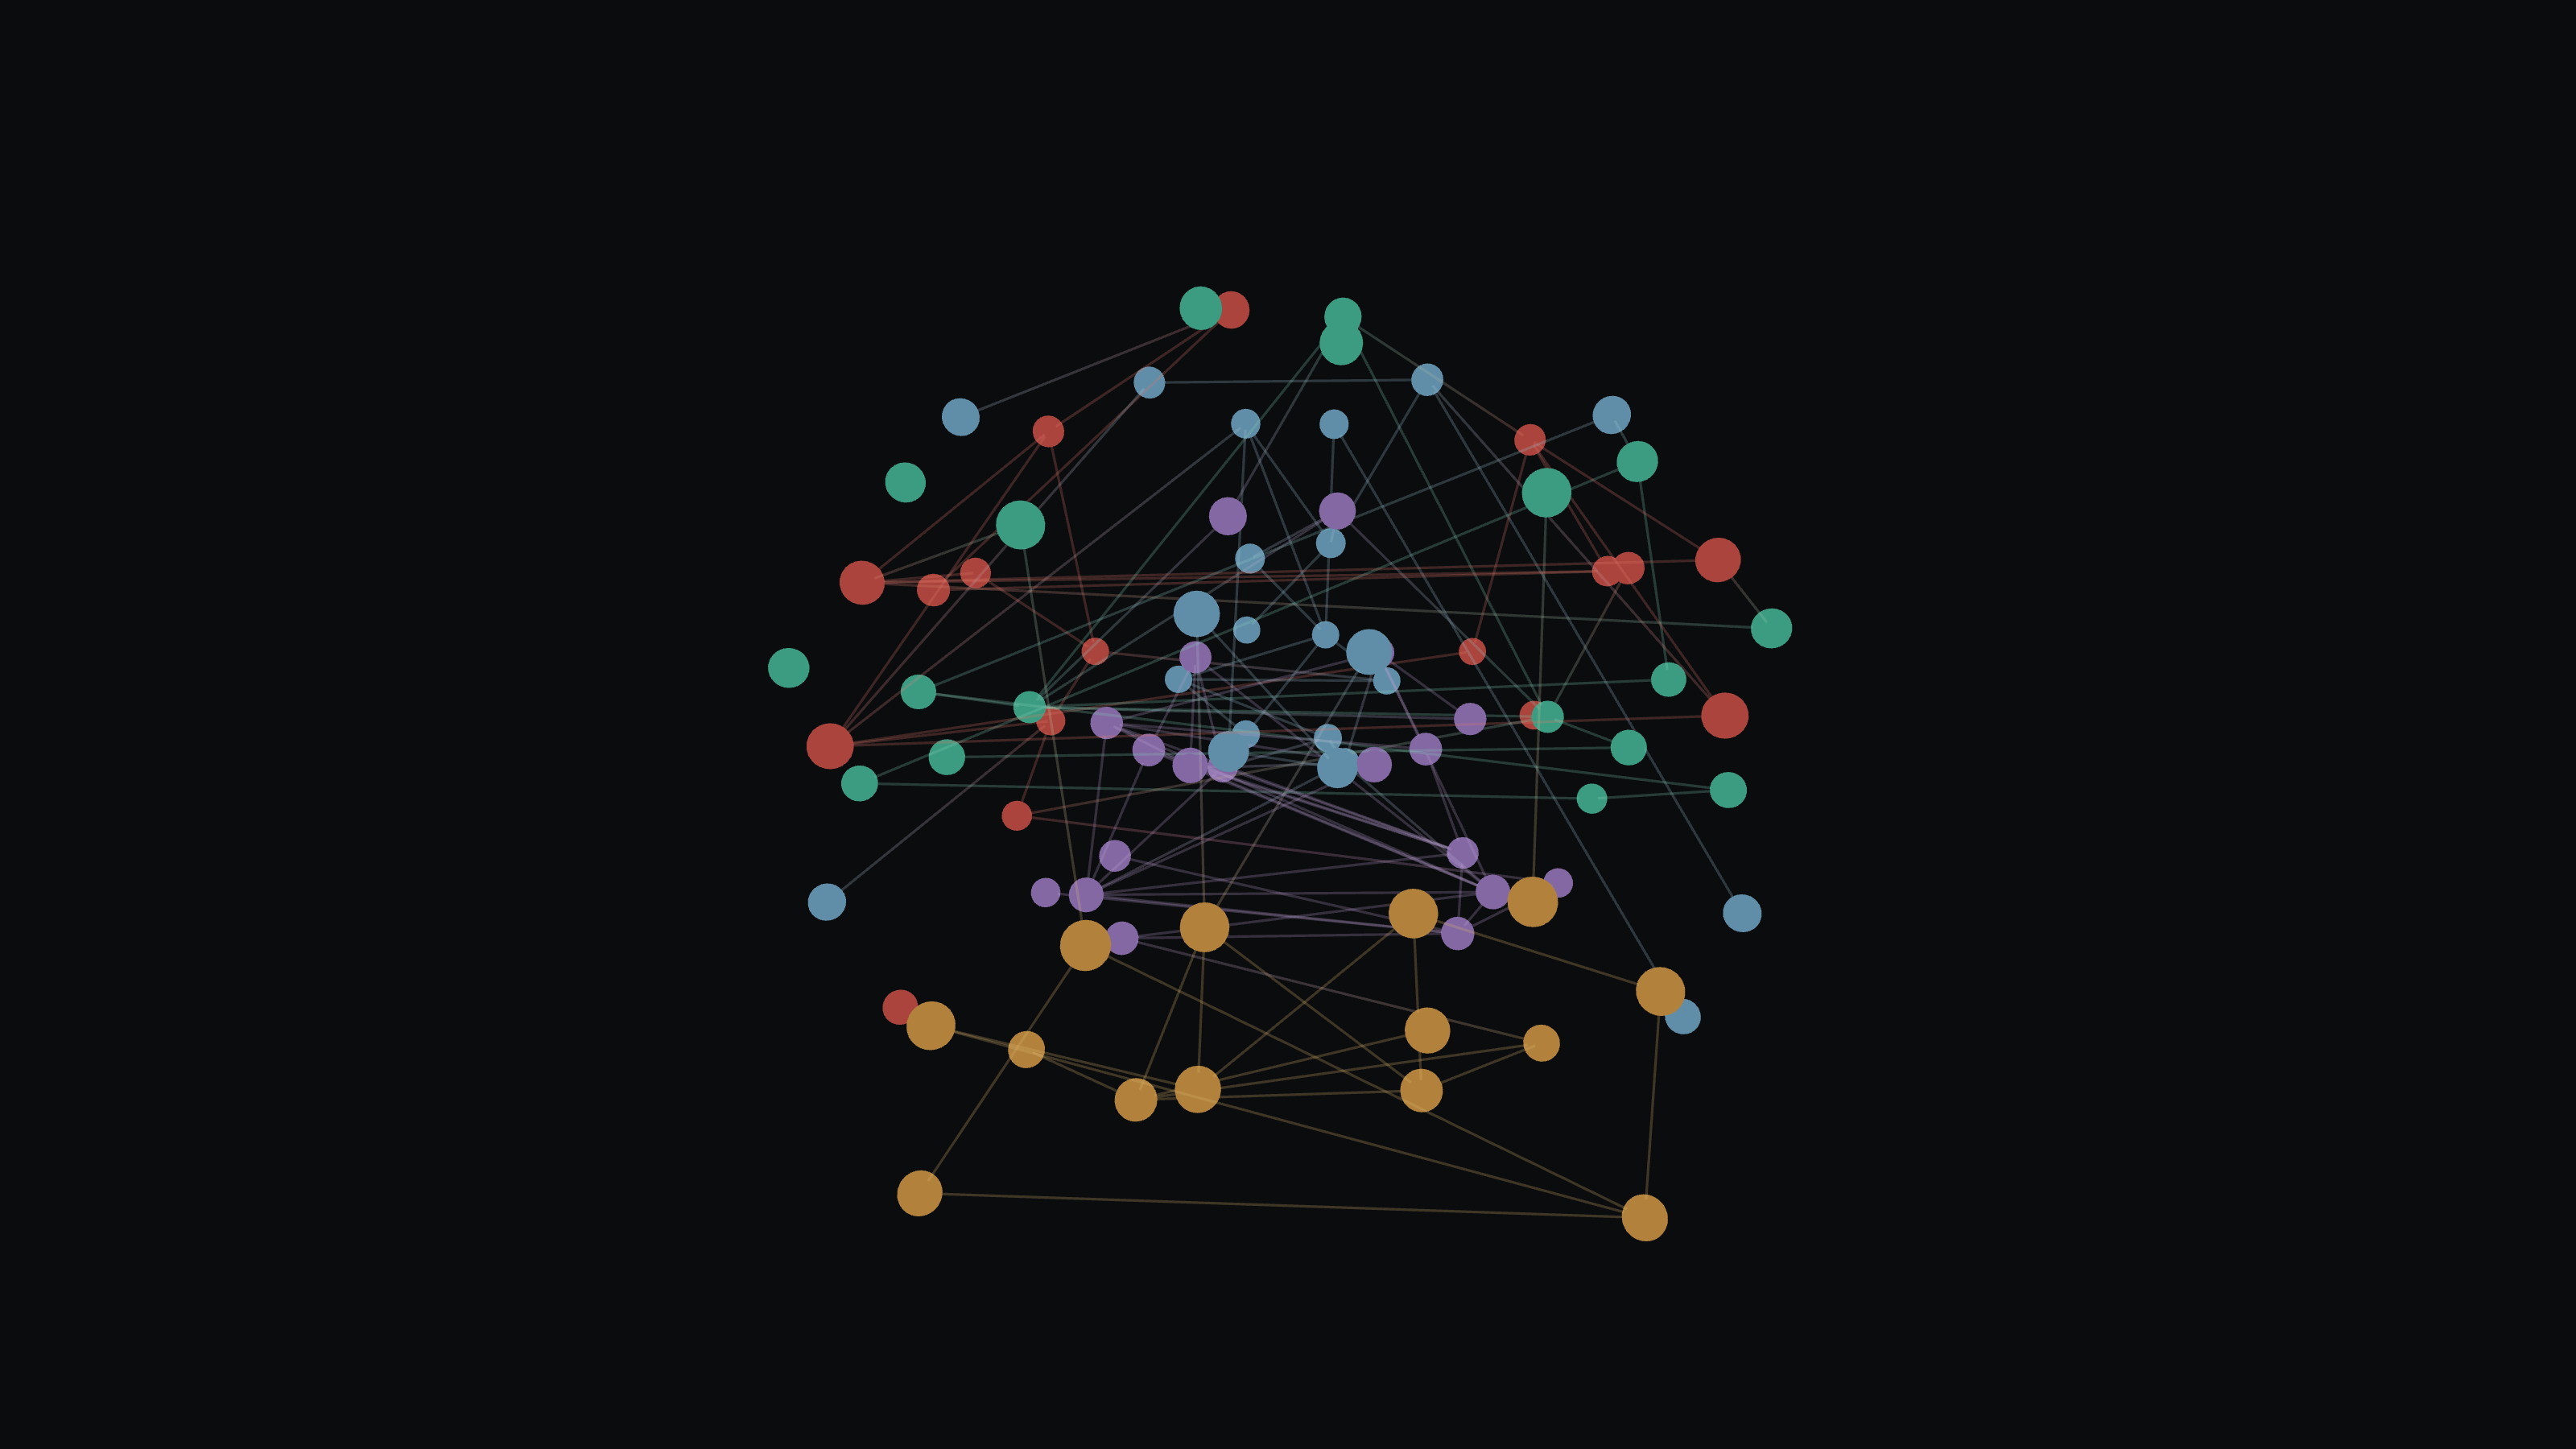
\includegraphics[height=\paperheight]{escena_umbral_70}};
		\end{scope}
		\draw[acento, line width=1.5pt]
			([xshift=0.5\paperwidth]current page.north west) --
			([xshift=0.5\paperwidth]current page.south west);
		% Texto de los dos primeros sprints, arriba, donde la escena está vacía
		\node[anchor=north, fill=fondo, fill opacity=0.9, text opacity=1, draw=linea,
		      rounded corners=6pt, inner sep=1.0em, text=texto, align=left,
		      text width=0.62\paperwidth]
			at ([yshift=-0.05\paperheight]current page.north)
			{{\large\bfseries Sprints 1 y 2}\quad
			 {\color{acentoclaro}\large\bfseries Ver la red y explorarla}\\[0.7em]
			 {\small Se leen los ficheros \texttt{.node} y \texttt{.edge} de \textbf{BrainNet
			 Viewer}, el formato que ya usa la gente del área, y los 90 nodos se dibujan en sus
			 \textbf{coordenadas anatómicas}.\\[0.4em]
			 El \textbf{umbral} deja solo las conexiones más intensas y saca la estructura a la
			 vista. Al tocar una región se resaltan sus conexiones y se muestran sus datos.}};
		\node[anchor=south west, fill=fondo, fill opacity=0.85, text opacity=1, inner sep=0.6em,
		      rounded corners=4pt, text=texto]
			at ([shift={(0.03\paperwidth,0.05\paperheight)}]current page.south west)
			{\small\bfseries Umbral 0,00\quad\suave{las 411 conexiones}};
		\node[anchor=south east, fill=fondo, fill opacity=0.85, text opacity=1, inner sep=0.6em,
		      rounded corners=4pt, text=texto]
			at ([shift={(-0.03\paperwidth,0.05\paperheight)}]current page.south east)
			{\small\bfseries Umbral 0,70\quad\suave{solo las más intensas}};
	\end{tikzpicture}
\end{frame}
\endgroup

% ======================================================= 7. RENDIMIENTO =====
\begin{frame}{El problema de rendimiento, y cómo se resolvió}
	\vspace{0.2em}
	\begin{columns}[T]
		\begin{column}{0.44\textwidth}
			{\color{rojo}\bfseries La primera versión}\\[0.5em]
			{\small Cada vez que se movía el control se recorrían todas las aristas y se reconstruía
			la geometría entera. El control iba a tirones.}\\[0.8em]
			{\color{ambar}\bfseries La propiedad que lo simplifica}\\[0.4em]
			{\small Si el servidor envía las aristas \textbf{ordenadas por peso}, las visibles son
			siempre \textbf{las primeras}.}
		\end{column}
		\begin{column}{0.52\textwidth}
			{\color{verde}\bfseries La solución}\\[0.4em]
			\begin{tikzpicture}[font=\scriptsize]
				\foreach \i in {0,...,5} \fill[verde] (\i*0.62, 0) rectangle (\i*0.62+0.46, 0.5);
				\foreach \i in {6,...,11} \fill[linea] (\i*0.62, 0) rectangle (\i*0.62+0.46, 0.5);
				\draw[acento, line width=1.4pt] (3.65,-0.2) -- (3.65,0.72);
				\node[text=acento, anchor=south, font=\scriptsize\bfseries] at (3.65,0.75) {umbral};
				\node[text=verde,   anchor=north, font=\scriptsize] at (1.6,-0.25) {se dibujan};
				\node[text=tenue,   anchor=north, font=\scriptsize] at (5.5,-0.25) {no se dibujan};
				\node[text=apagado, anchor=west,  font=\scriptsize] at (0,1.15)
					{aristas ordenadas por peso, de mayor a menor};
			\end{tikzpicture}
			\vspace{0.5em}
			\begin{itemize}
				\setlength{\itemsep}{0.2em}
				\item[] {\small La geometría se construye \clave{una sola vez}.}
				\item[] {\small Filtrar es decir \clave{cuántas dibujar}: coste constante.}
				\item[] {\small Cuántas son, con \clave{búsqueda binaria}: $O(\log E)$.}
			\end{itemize}
		\end{column}
	\end{columns}
\end{frame}

% ======================================================== 8. REVISIONES =====
\begin{frame}{Lo que salió de las revisiones}
	\vspace{0.4em}
	\begin{columns}[T]
		\begin{column}{0.31\textwidth}
			\tarjeta[rojo]{Conexiones más gruesas}{Parecía cambiar un número. WebGL no obliga a
				dibujar líneas de más de un píxel: hubo que cambiar la forma de dibujarlas.}
		\end{column}
		\begin{column}{0.31\textwidth}
			\tarjeta[ambar]{El grado, con el umbral}{El de la red completa deja de ser lo que se
				está viendo. Ahora el panel dice, por ejemplo, 2 conexiones visibles de 9.}
		\end{column}
		\begin{column}{0.31\textwidth}
			\tarjeta[verde]{Resaltar sin desteñir}{Las conexiones del nodo elegido se distinguen
				manteniendo su color, en lugar de teñirse de azul.}
		\end{column}
	\end{columns}
	\vspace{1.0em}
	\begin{center}
		\suave{\small Ninguna se me habría ocurrido probando yo solo la aplicación, precisamente
		porque yo ya sabía lo que hacía cada cosa.}
	\end{center}
\end{frame}

% ======================================== 9. SPRINT 3 Y SUS COMPROBACIONES ===
\begin{lienzo}{escena_intermediacion}
	\sobreimagen[north east]{-0.045\paperwidth,-0.07\paperheight}{%
		{\Large\bfseries Sprint 3}\ \ {\color{acentoclaro}\large\bfseries Analizar la red}\\[0.7em]
		{\small
		\textbf{Cuatro métricas globales} y \textbf{tres centralidades} por región. El tamaño y el
		color de cada nodo representan la métrica elegida: aquí, la intermediación.\\[0.6em]
		{\color{acentoclaro}\bfseries ¿Y cómo sé que están bien?}\\[0.3em]
		Contrasté las cinco con implementaciones escritas por mí sin la librería, incluida una del
		\textbf{algoritmo de Brandes}.\\[0.4em]
		Comprobar que la suma de los grados fuera el doble del número de aristas destapó un
		\textbf{error real} que \textbf{no daba ningún síntoma en pantalla}.}}
\end{lienzo}

% ========================================= 10. SPRINT 4 Y SU IMPACTO ========
\begin{lienzo}{app_catalogo}
	\sobreimagen[north west]{0.045\paperwidth,-0.07\paperheight}{%
		{\Large\bfseries Sprint 4}\ \ {\color{acentoclaro}\large\bfseries Un sistema con
		usuarios}\\[0.7em]
		{\small
		Cuentas, \textbf{redes propias} que solo ve quien las sube, exportación en CSV y JSON y
		panel de \textbf{administración}.\\[0.6em]
		{\color{acentoclaro}\bfseries El sistema deja de ser sin estado}\\[0.3em]
		Las contraseñas no se guardan, se guarda un resumen. La sesión va firmada en una cookie que
		el navegador impide leer. Y toda consulta filtra por el usuario: nunca se confía en lo que
		pida el cliente.\\[0.4em]
		Fue lo primero que cubrí con pruebas automáticas.}}
\end{lienzo}

% ======================================================== 11. PUBLICARLA =====
\begin{frame}{Publicarla, y que se vea en cualquier pantalla}
	\vspace{0em}
	\begin{columns}[T]
		\begin{column}{0.45\textwidth}
			\tarjeta[rojo]{Lo que tenía}{Dos contenedores que se hablaban por un nombre interno de
				Docker, con servidores de desarrollo. Servía para trabajar, no para publicar.}\\[0.6em]
			\tarjeta[verde]{Lo que hice}{Una imagen en dos etapas: una compila la interfaz y otra la
				sirve desde el propio servidor. Todo en un solo contenedor, ya publicado.}
		\end{column}
		\begin{column}{0.51\textwidth}
			\centering
			\begin{tikzpicture}
				\node[draw=linea, line width=1pt, rounded corners=8pt, inner sep=0pt]
					{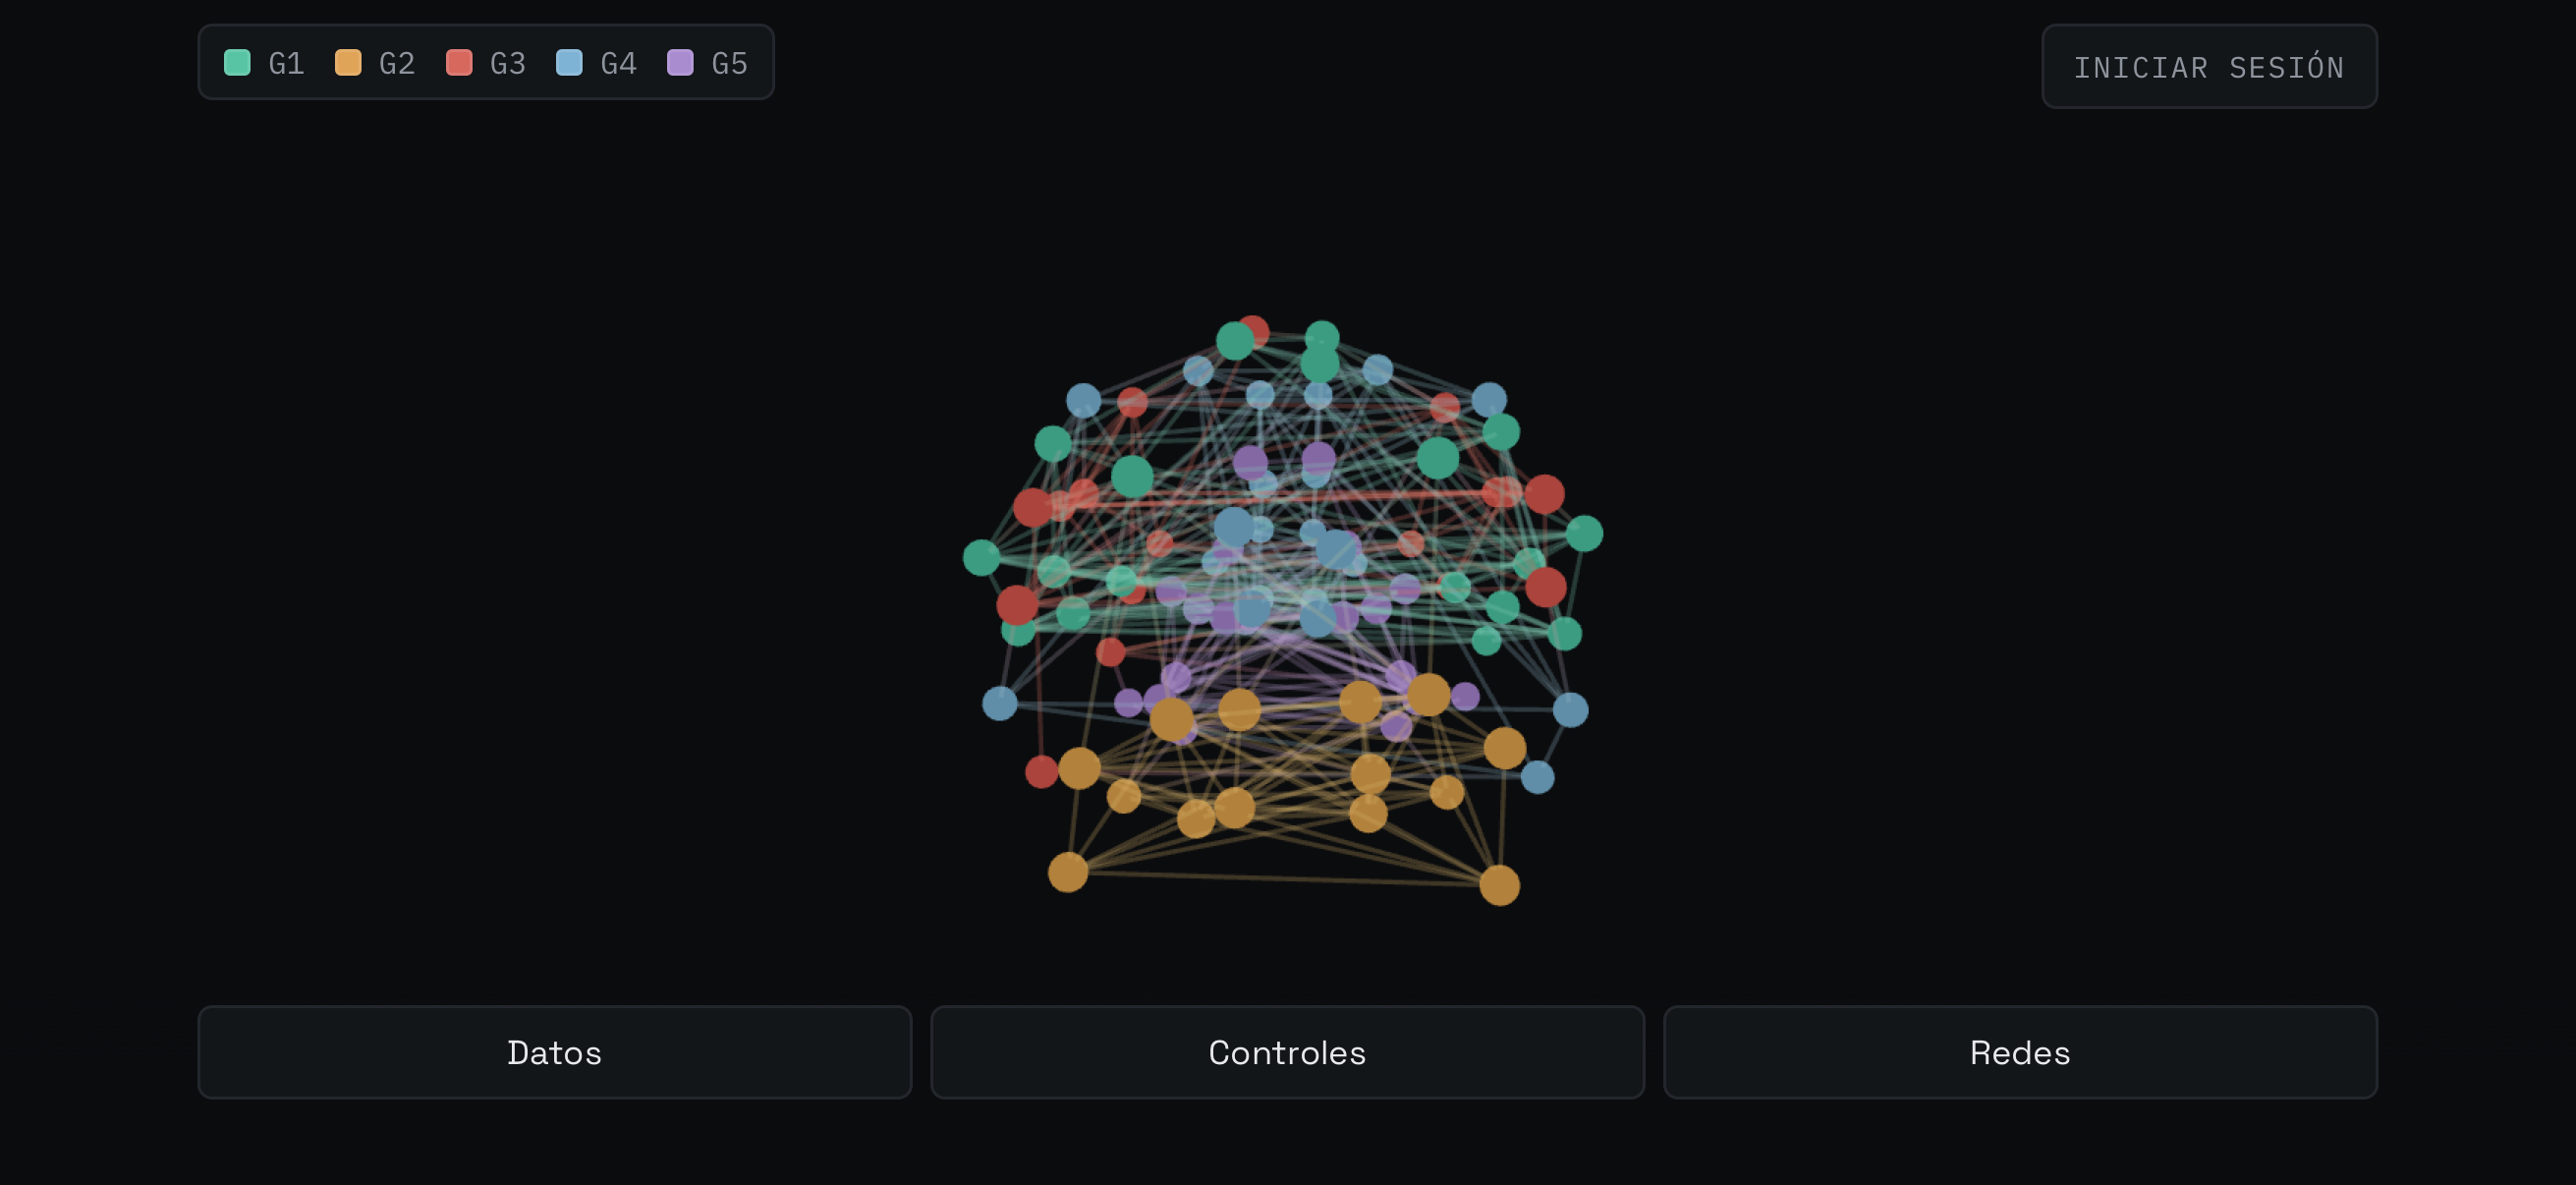
\includegraphics[width=0.49\paperwidth]{app_movil_horizontal}};
			\end{tikzpicture}\\[0.4em]
			{\footnotesize En el móvil los paneles se abren desde una barra: cambia \clave{cuándo se
			muestran}, no cuánto ocupan.}\\[0.3em]
			{\color{tenue}\scriptsize El criterio no puede ser solo el ancho: girado tiene ancho de
			sobra y casi nada de altura.}
		\end{column}
	\end{columns}
\end{frame}

% ========================================================= 12. VALIDACIÓN =====
\begin{frame}{Validación}
	\vspace{0.9em}
	\begin{center}
		\cifra{17}{pruebas automáticas, en una orden}\hfill
		\cifra[verde]{32}{pruebas de aceptación, una por requisito}\hfill
		\cifra[ambar]{5}{métricas contrastadas con código propio}
	\end{center}
	\vspace{1.6em}
	\begin{columns}[T]
		\begin{column}{0.46\textwidth}
			{\color{verde}\bfseries Rendimiento}\\[0.4em]
			{\small Multiplicar por treinta el número de conexiones \clave{no produjo degradación
			apreciable} en el dibujado.}
		\end{column}
		\begin{column}{0.46\textwidth}
			{\color{ambar}\bfseries Lo que dejo señalado}\\[0.4em]
			{\small La comprobación formal de los 60 fotogramas por segundo no la doy por buena: el
			mismo resultado salía midiendo una página vacía.}
		\end{column}
	\end{columns}
\end{frame}

% ============================================================= 13. DEMO =====
\begingroup
\usebackgroundtemplate{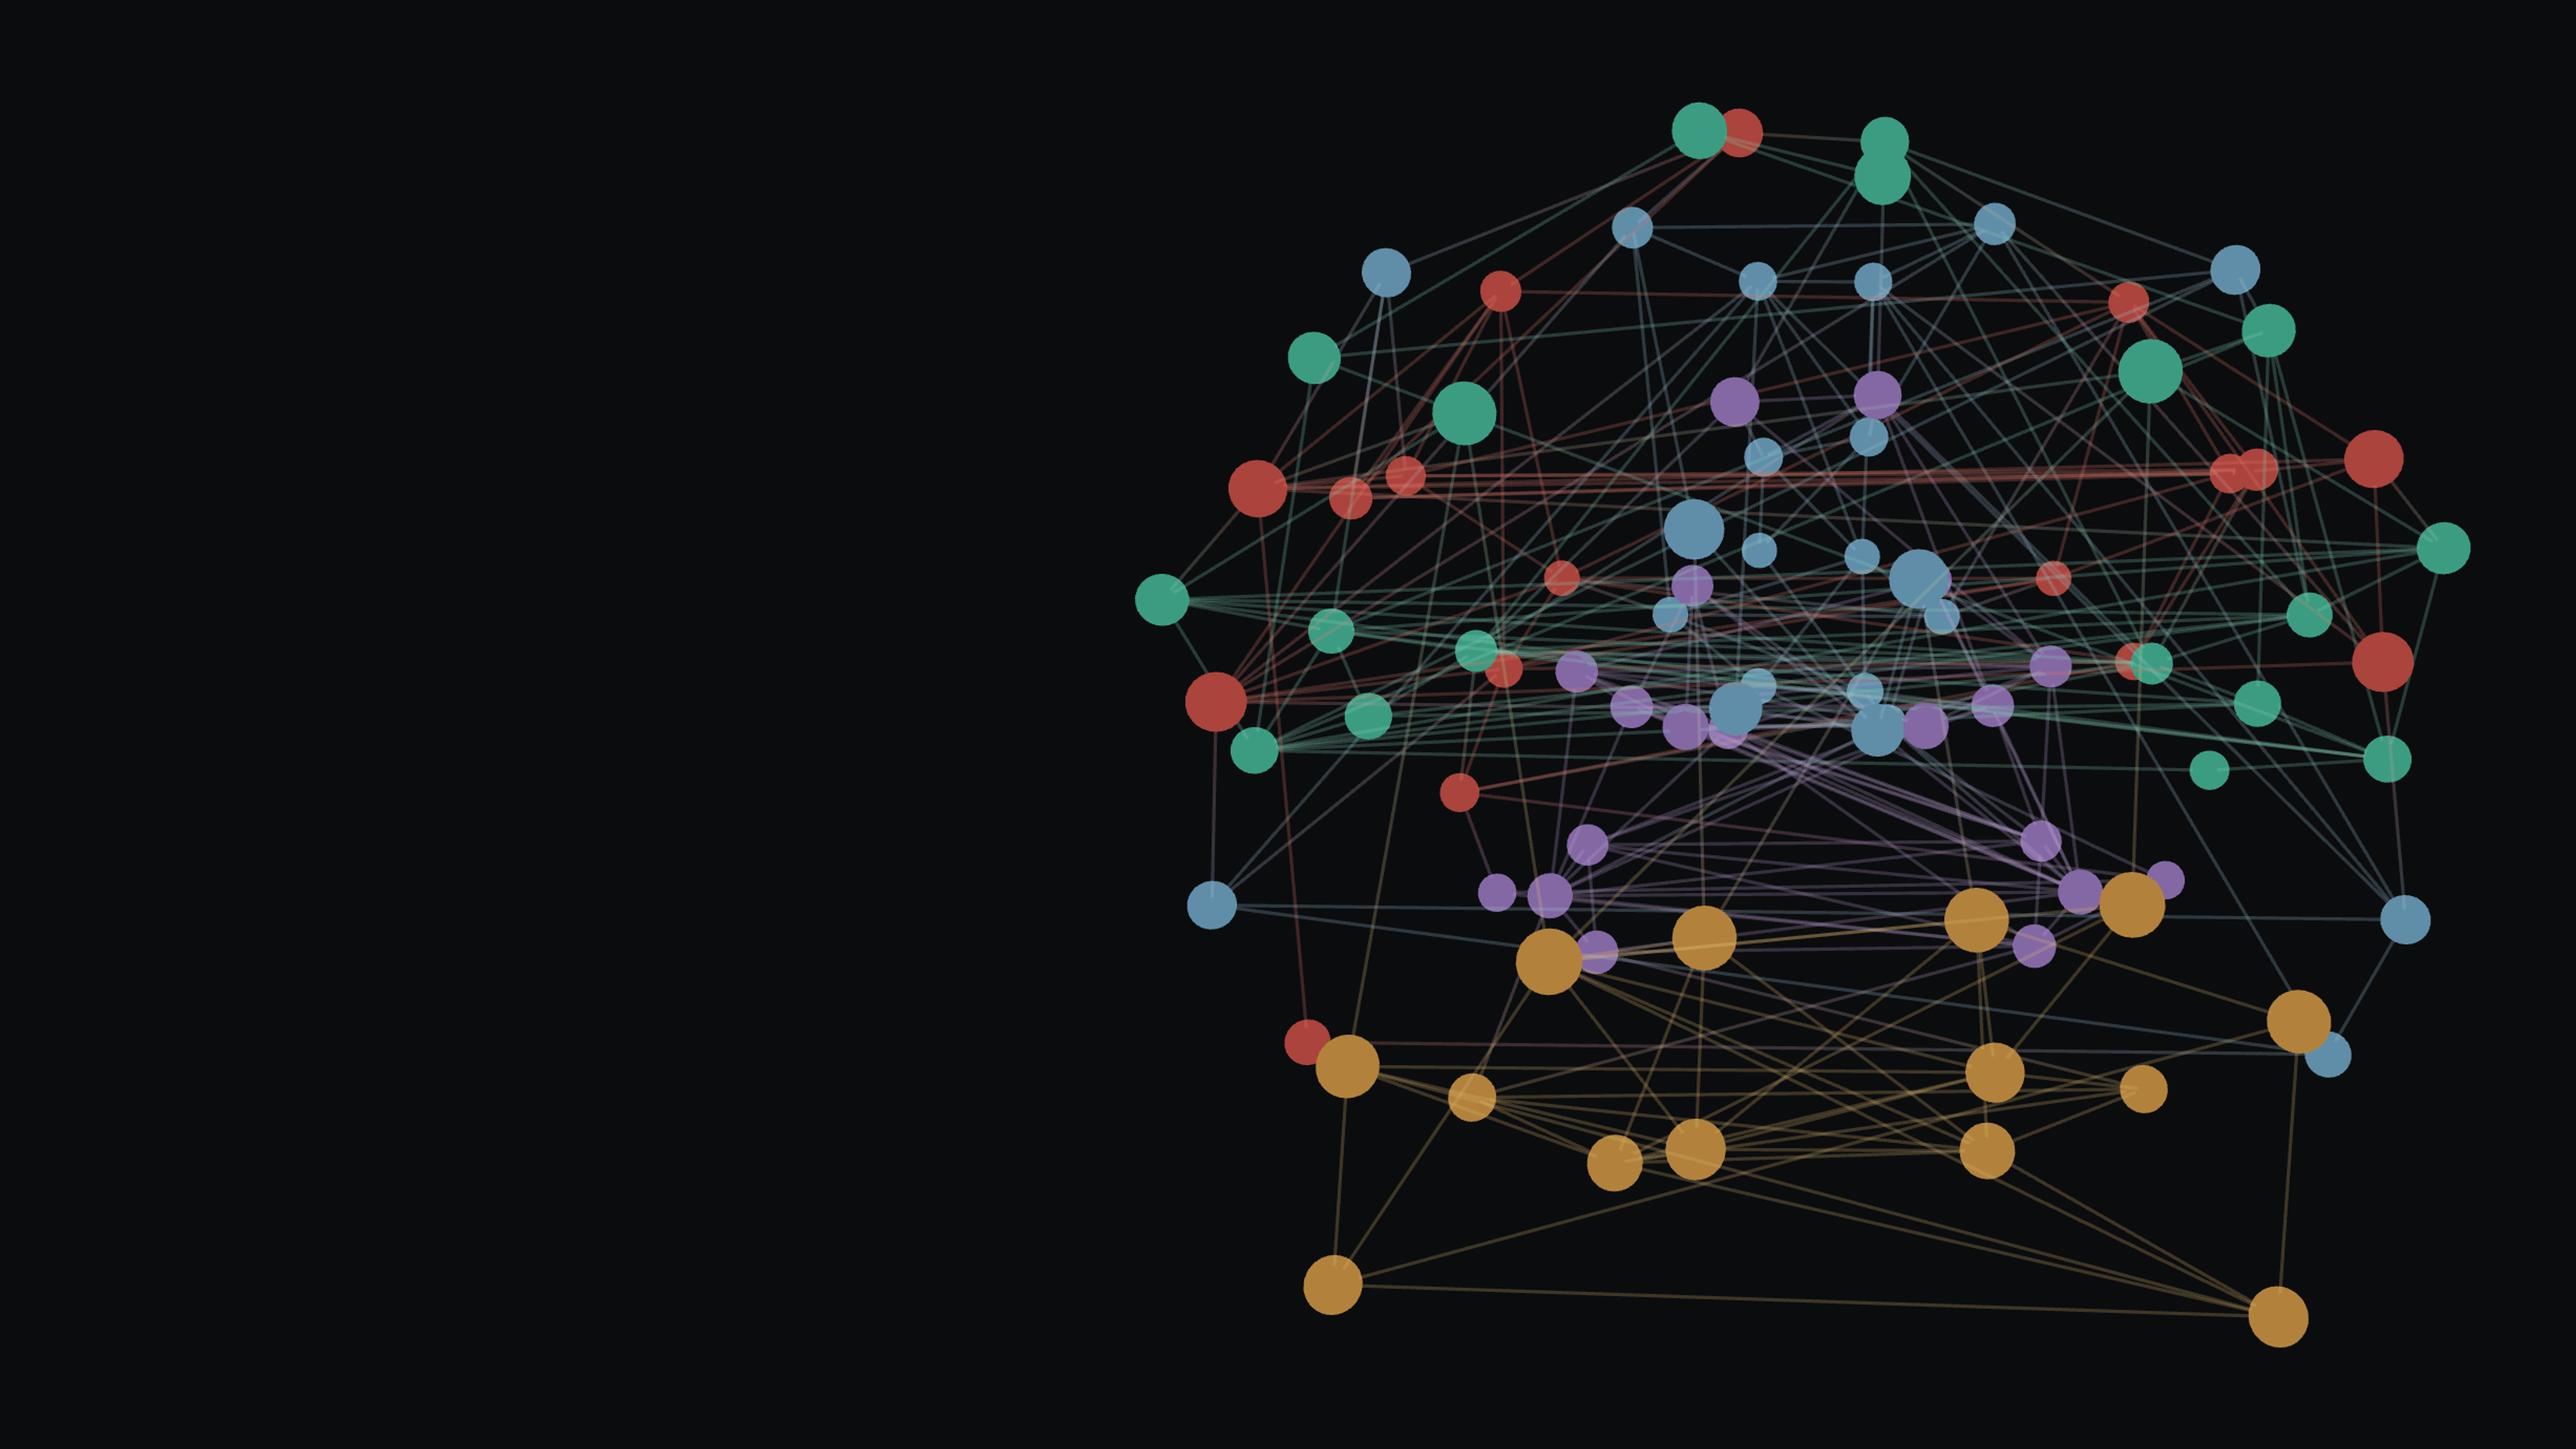
\includegraphics[width=\paperwidth, height=\paperheight]{hero}}
\begin{frame}[plain]
	\veloizq
	\begin{tikzpicture}[remember picture, overlay]
		\node[anchor=west, align=left, text width=0.42\paperwidth]
			at ([xshift=0.075\paperwidth]current page.west) {%
			{\color{acento}\rule{3.5em}{2.5pt}}\\[1.1em]
			{\color{texto}\fontsize{34}{38}\selectfont\bfseries Demostración}\\[1.1em]
			{\color{apagado}\texttt{brain-viz.onrender.com}}};
	\end{tikzpicture}
\end{frame}
\endgroup

\section{Conclusiones}

% ===================================================== 15. CUMPLIMIENTO =====
\begin{frame}{Grado de cumplimiento}
	\vspace{0.4em}
	\begin{center}
		\begin{tikzpicture}[font=\small]
			\foreach \i/\t/\e in {%
				0/{Cargar y visualizar redes en 3D de forma interactiva}/{Sprint 1},
				1/{Análisis con métricas de teoría de grafos}/{Sprint 3},
				2/{Navegar, filtrar, seleccionar e inspeccionar}/{Sprints 2 y 3},
				3/{Mantenible, con el procesamiento separado de la vista}/{Los cuatro sprints},
				4/{Despliegue sencillo}/{Cumplido, con matices}} {
				\node[text=verde, anchor=west, font=\normalsize\bfseries] at (0, -\i*0.92) {$\checkmark$};
				\node[text=texto, anchor=west] at (0.55, -\i*0.92) {\t};
				\node[text=apagado, anchor=east, font=\footnotesize] at (11.6, -\i*0.92) {\e};
				\draw[linea] (0,-\i*0.92-0.34) -- (11.6,-\i*0.92-0.34);
			}
		\end{tikzpicture}
	\end{center}
	\vspace{0.7em}
	\begin{center}\small
		Los \clave{18 requisitos funcionales} están implementados, junto con los no funcionales y
		los de información.
	\end{center}
\end{frame}

% ============================== 16. LO QUE ME LLEVO Y TRABAJO FUTURO ========
\begin{frame}{Lo que me llevo, y lo que queda por hacer}
	\vspace{0.5em}
	\begin{columns}[T]
		\begin{column}{0.47\textwidth}
			{\color{apagado}\scriptsize LO QUE ME LLEVO}\\[0.7em]
			{\small
			\begin{itemize}
				\setlength{\itemsep}{0.6em}
				\item Buscar la \clave{propiedad de los datos} rinde más que optimizar el código.
				\item Las pruebas no son un trámite: el error del grado \clave{no se veía}.
				\item «Terminado» no es «funciona»: el buscador filtraba bien y no servía.
				\item Las revisiones cambiaron el resultado más de lo que esperaba.
			\end{itemize}}
		\end{column}
		\begin{column}{0.47\textwidth}
			{\color{apagado}\scriptsize TRABAJO FUTURO}\\[0.7em]
			{\small
			\begin{itemize}
				\setlength{\itemsep}{0.6em}
				\item Detectar \clave{comunidades}, camino más corto y comparar dos redes.
				\item Admitir \clave{más formatos y atlas}, sin convertir nada a mano.
				\item Compartir una red con personas concretas y enviar enlaces a una vista.
				\item \clave{Accesibilidad}: depende mucho del color y no está probada.
			\end{itemize}}
		\end{column}
	\end{columns}
\end{frame}

% =========================================================== 17. CIERRE =====
\begingroup
\usebackgroundtemplate{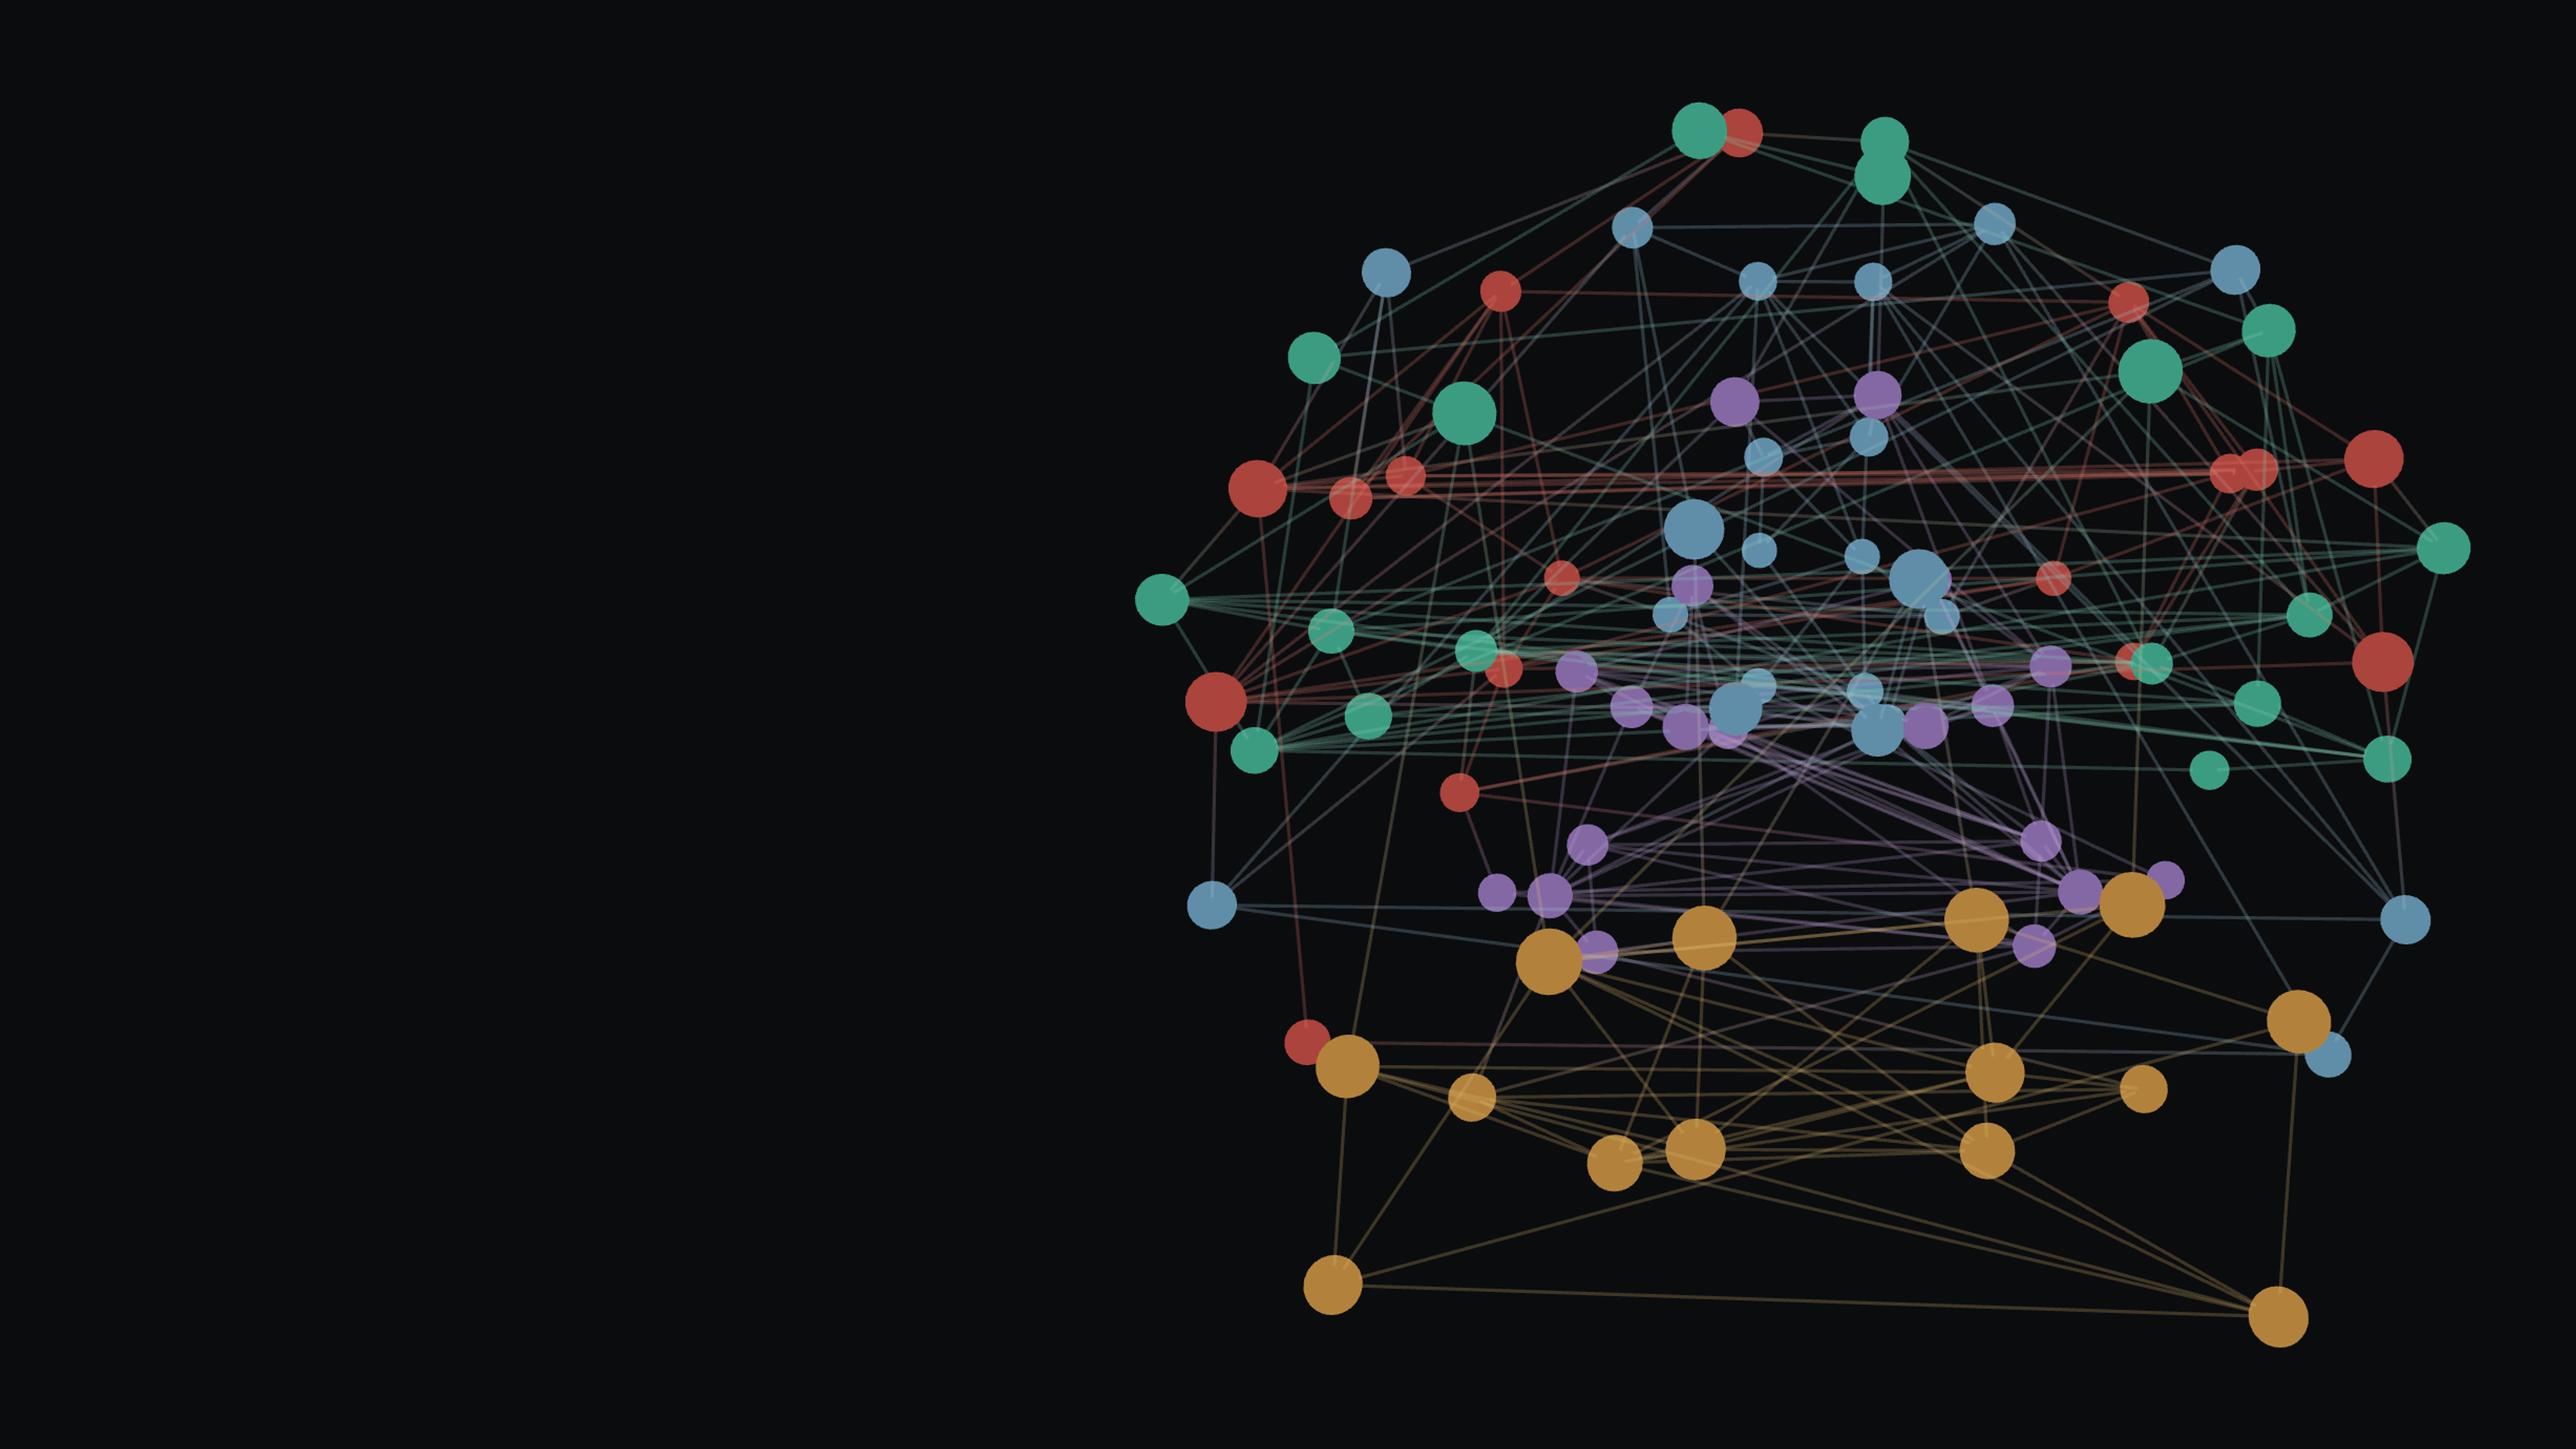
\includegraphics[width=\paperwidth, height=\paperheight]{hero}}
\begin{frame}[plain]
	\veloizq
	\begin{tikzpicture}[remember picture, overlay]
		\node[anchor=west, align=left, text width=0.44\paperwidth]
			at ([xshift=0.075\paperwidth]current page.west) {%
			{\color{texto}\fontsize{30}{34}\selectfont\bfseries Gracias por\\ su atención}\\[1.2em]
			{\color{acento}\rule{3.5em}{2.5pt}}\\[1.3em]
			
\includegraphics[width=0.075\paperwidth]{qr_app}\\[0.6em]
			{\color{acentoclaro}\small\texttt{brain-viz.onrender.com}}\\[1.5em]
			{\color{tenue}\footnotesize Pablo Moliz Arias\\ Tutor: Juan Ruiz de Miras}};
	\end{tikzpicture}
\end{frame}
\endgroup

% =================================================== 18 a 25. RESERVA =======
\begin{frame}[plain, noframenumbering]
	\vfill
	\begin{center}
		{\color{tenue}\rule{3em}{1.5pt}}\\[0.9em]
		{\color{apagado}\Large Diapositivas de reserva}
	\end{center}
	\vfill
\end{frame}

\begin{frame}[noframenumbering]{Reserva: el montaje de desarrollo}
	\centering\diagrama[0.58\textheight]{arquitectura}\\[0.2em]
	\suave{\scriptsize Dos contenedores en desarrollo. Al publicarla pasa a uno solo.}
\end{frame}

\begin{frame}[noframenumbering]{Reserva: modelo de datos}
	\centering\diagrama[0.62\textheight]{clases_sprint4}
\end{frame}

\begin{frame}[noframenumbering]{Reserva: módulos del sistema}
	\centering\diagrama[0.62\textheight]{modulos_sprint4}
\end{frame}

\begin{frame}[noframenumbering]{Reserva: qué ocurre al mover el umbral}
	\centering\diagrama[0.62\textheight]{sec_interaccion_sprint2}
\end{frame}

\begin{frame}[noframenumbering]{Reserva: planificación y coste}
	\vspace{1.4em}
	\begin{center}
		\cifra{38}{días laborables}\hfill
		\cifra[verde]{300 h}{de trabajo}\hfill
		\cifra[ambar]{4.968\,\euro}{coste estimado}
	\end{center}
	\vspace{2.0em}
	\begin{center}
		\begin{minipage}{0.8\paperwidth}\small
			El reparto por sprints no fue el previsto. Estimé cinco días para el Sprint 4, el menor
			de los cuatro, y resultó el más largo: era el único que introducía cosas que no existían
			en el proyecto, como la base de datos y las cuentas. Los tres primeros ampliaban algo
			que ya funcionaba; el cuarto cambió la arquitectura.
		\end{minipage}
	\end{center}
\end{frame}

\begin{frame}[noframenumbering]{Reserva: cifras de la red y coste de las métricas}
	\vspace{0.9em}
	\begin{columns}[T]
		\begin{column}{0.44\textwidth}
			\begin{tikzpicture}[font=\small]
				\foreach \i/\m/\v in {0/Nodos/90, 1/Conexiones/411, 2/Densidad/{0,103},
				                      3/{Grado medio}/{9,13}, 4/{Agrupamiento}/{0,548},
				                      5/{Componentes}/1} {
					\node[text=apagado, anchor=west] at (0, -\i*0.8) {\m};
					\node[text=texto, anchor=east, font=\small\bfseries] at (5.4, -\i*0.8) {\v};
					\draw[linea] (0,-\i*0.8-0.3) -- (5.4,-\i*0.8-0.3);
				}
			\end{tikzpicture}
		\end{column}
		\begin{column}{0.5\textwidth}
			{\color{apagado}\scriptsize COSTE DE LA INTERMEDIACIÓN}\\[1.2em]
			\begin{tikzpicture}[font=\scriptsize]
				\node[text=texto, anchor=west, font=\scriptsize] at (0,2.3) {500 nodos, primera vez};
				\fill[rojo] (0,1.5) rectangle (5.4,1.98);
				\node[text=rojo, anchor=west, font=\small\bfseries] at (5.55,1.74) {652 ms};
				\node[text=texto, anchor=west, font=\scriptsize] at (0,1.15) {ya calculada};
				\fill[verde] (0,0.35) rectangle (0.24,0.83);
				\node[text=verde, anchor=west, font=\small\bfseries] at (0.4,0.59) {4 ms};
				\node[text=apagado, anchor=west, font=\scriptsize] at (0,-0.3)
					{se guarda procesada: 147 veces más rápido};
			\end{tikzpicture}
		\end{column}
	\end{columns}
\end{frame}

\begin{frame}[noframenumbering]{Reserva: la interfaz en un teléfono}
	\centering
	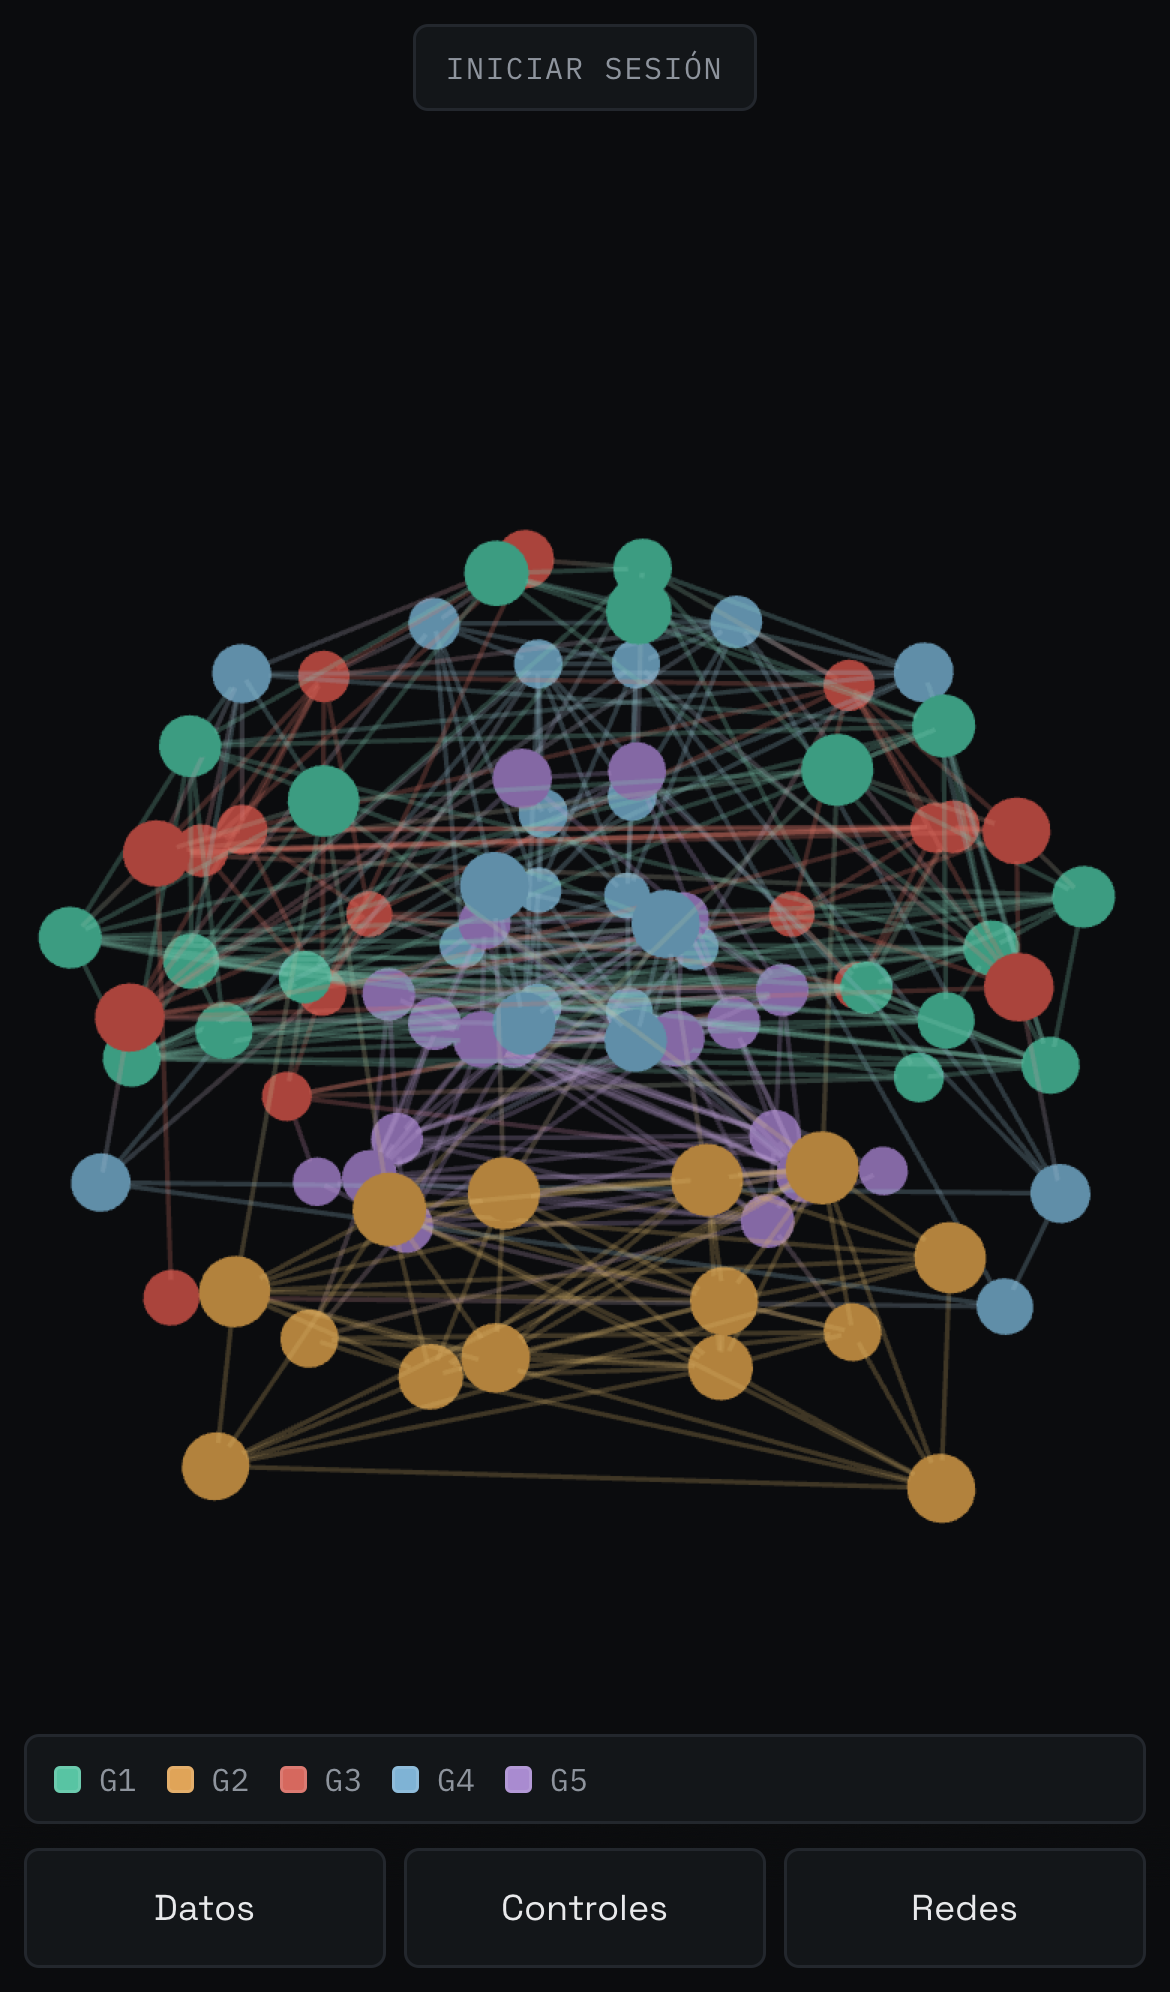
\includegraphics[height=0.66\textheight]{app_movil_escena}\hspace{1.5em}
	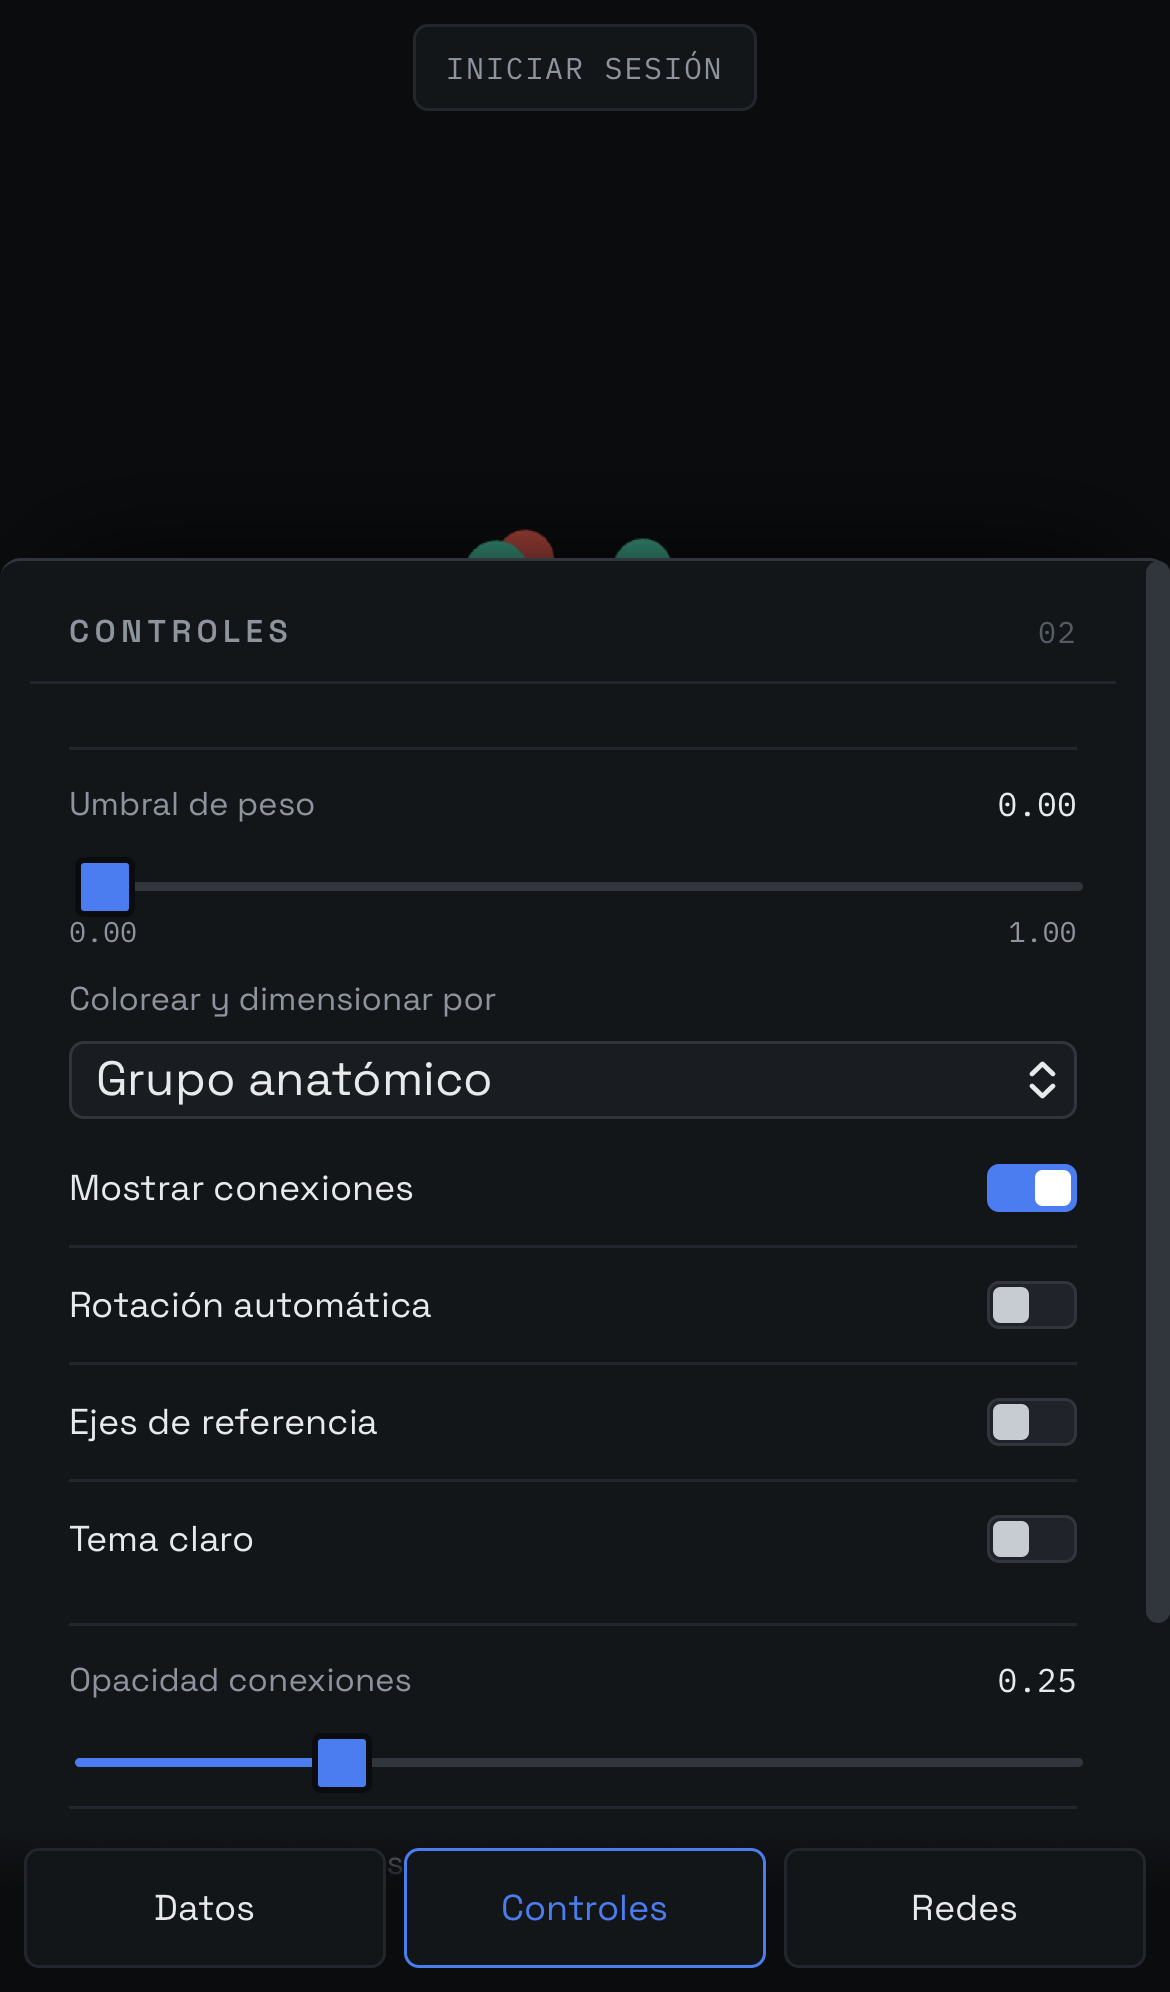
\includegraphics[height=0.66\textheight]{app_movil_hoja}
\end{frame}

\end{document}
